%\documentclass{article}
%\usepackage{preamble}
%
%\title{Signal and Transforms Samanfattning}
%\author{Anton Augustsson}
%%\date{Octrober 2021}
%
%
%\begin{document}
%
%\maketitle
%\newpage
%\tableofcontents
%\newpage

\chapter{Signal and Transforms}

\newpage

\section{Introduction}
\subsection{System Clasification}
%\href{https://www.youtube.com/watch?v=e967IQA7dDI}{1.1 signal introduction and classification}
%\begin{center}
%\begin{tabular}{ | c c | c c | c c |}
%    \hline
% Continuous time & discreate time & periodic & Aperiodic & even & odd \\
% $x(t)$ & $x[k]$ & $x(t)=x(t+T)$ & none & $x_e(t) = x_e(-t)$ & $x_0(t)=-x_0(-t)$ \\
% Analog signal  & digital signal & T-period & none & Abbsolut value, cos & sin, negative t positve t \\
%  & & sin,cos & & & \\
%    \hline
%\end{tabular}
%\end{center}

\begin{itemize}
    \item \textit{Continuos-time}: Defined for a all times in a time period $x(t)$
    \item \textit{Discrete-time}: Defined for a some times in a time period $x[k]$
    \item \textit{Analog}: Continous time signal time-varing 
    \item \textit{Digital}: Discreate time signal
    \item \textit{Linear/ Non-linear}: if $\alpha x_1(t) + \beta x_2(t) \mapsto \alpha y_1(t) + \beta y_2(t)$ (supper position)
    \item \textit{Periodic/ Aperiodic}: $x(t)=x(t+T)$
    \item \textit{Casual}: time dependent on on previus not next values
    \item \textit{time-varieng/ time-invariant} $x(t-T) \mapsto y(t-T)$
    \item \textit{Deterministic} Same result each time no random.
    \item \textit{stochastic} random -signals (won't look at)
    \item \textit{Stable/ unstable}  bounded $lim_{t\to\infty} x(t) < \infty$
    \item \textit{Invertible} Can invert
    \item \textit{SISO} (signal inlput signal output)
    \item \textit{MIMO} (multiple input multiple output)
    \item \textit{BIBO} (bounded input-bounded output) stable/undtable
\end{itemize}

\begin{center}
\begin{tabular}{ | c | c |}
    \hline
    \textbf{Linear, time invariant (LTI)} & Linear, time variant \\
    \hline
    non-linear, time invariant (LTI) & non-linear, time variant \\
    \hline
\end{tabular}
\end{center}

We only look at \underline{LTI only}.


\begin{figure}[H]
    \centering
    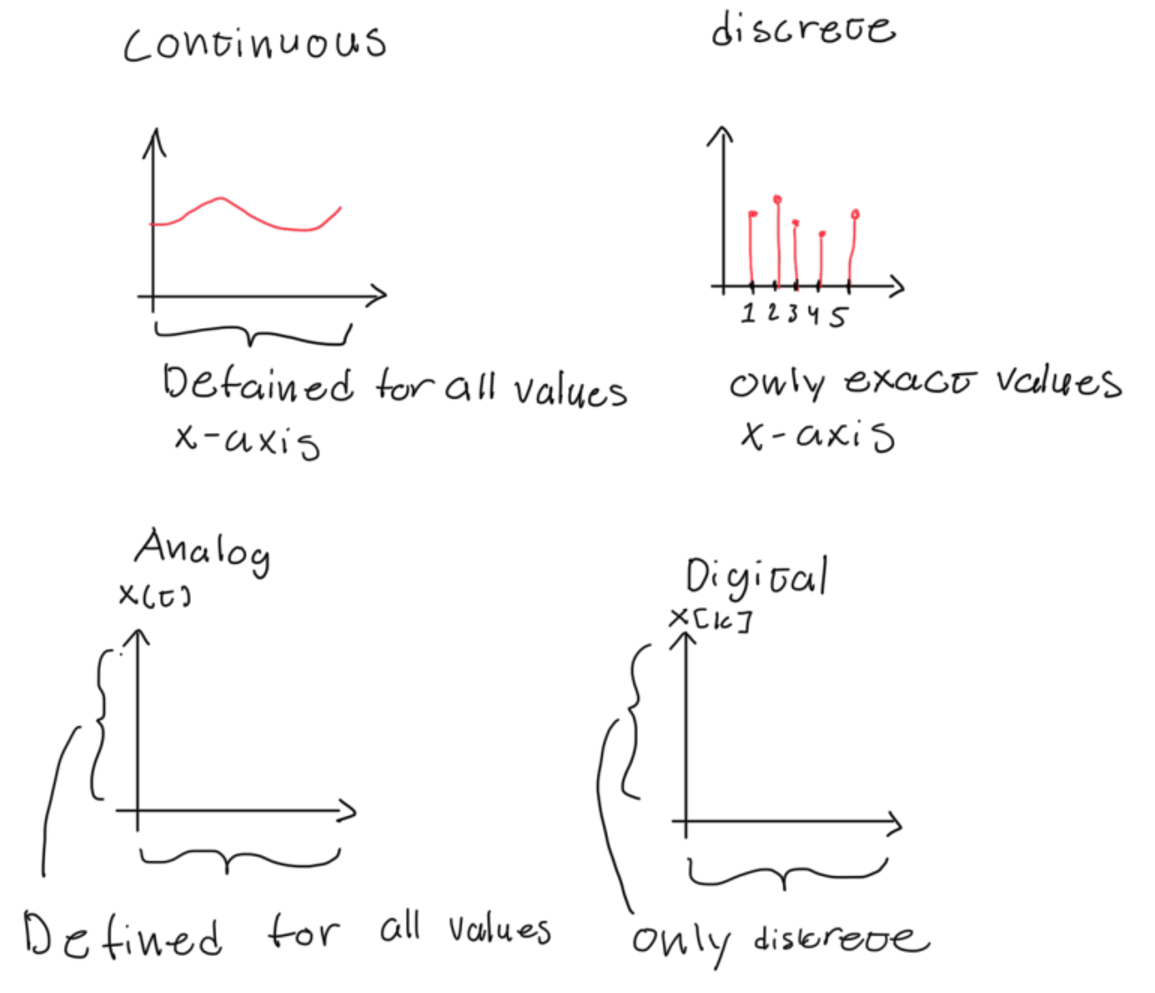
\includegraphics[width=12cm]{image/caractaristic-signal-plots.pdf}
    \caption{Signal plots}
\end{figure}

\begin{multicols}{2}
Anny signal can be expressed by its even and odd componetnt
\begin{equation}
    x(t) = x_e(t) + x_o(t)
\end{equation}

\textit{Sampling}: continuous time signal.
\begin{equation}
    x[k] \delequal x(k T_s)
\end{equation}
$T_s$ is the sampling time.
`The discreate signals at time $k$ equals to 
the continuous time signal $x(t)$ at time $t = kT_s$'.

\begin{align}
    x(t)  &\mapsto y(t)    \\
    x[t]  &\mapsto y[t]
\end{align}


\subsubsection{Transform methods}
A transform is a operator $\Tau\{ \dot \}$ from one domain to another.
\begin{equation*}
    X(\varsigma) = \Tau\{ x(t) \}
\end{equation*}

$x(t)$ and $X(\varsigma)$ are a \textit{transform pairs}
\begin{equation*}
    x(t) \TransformHoriz X(\varsigma)
\end{equation*}

The inverse transform $\Tau^{-1}\{ \dot \}$ restores the original signal.
\begin{equation*}
    x(t) = \Tau^{-1}\{ X(\varsigma) \}
\end{equation*}

\begin{exampleblock}{Example: Linear}
Is $\frac{dy(t)}{dt}+3ty(t)=t^2x(t)$ linear? Assume zero initial conditions.

\textbf{Solution:}
\begin{align*}
    &\frac{dy(t)}{dt}+3ty(t) = t^2x(t) \\
    &\frac{d(\alpha y_1(t) + \beta y_2(t))}{dt} + 3t(\alpha y_1(t) + \alpha y_2(t)) \\ 
    &= t^2(\alpha x_1(t) + \beta x_2(t)) \\
    &\alpha\frac{dy_1(t)}{dt} + \beta\frac{dy_2(t)}{dt} + \alpha 3ty_1(t) \beta 3ty_2(t) \\
    &= \alpha t^2 x_1(t) + \beta t^2 x_2(t)
\end{align*}
therefore is the system linear.
\end{exampleblock}


\begin{exampleblock}{Example: Time invariant}
Is $y(t)=tx(t-2)$ time invariant? 

\textbf{Solution:}
\begin{equation*}
    y(t-\tau) = tx((t-\tau)-2 \neq (t-\tau)x((t-\tau)-2 \\
\end{equation*}
therefore is the system time variant.
\end{exampleblock}

\vspace{1cm}
\begin{exampleblock}{Example: Casual}
Is $y(t)=x(-t)$ casual? 

\textbf{Solution:}
When $t<0$ then $t<-t$ with is not allowed in a casual system since it then depends on
upcoming values. If we were to restrict that $t\geq0$ then it would be casual.
\end{exampleblock}


\noindent\textbf{Euler's identities}
\begin{align*}
  e^{+jx} &= \cos{x} + j\sin{x} \\
  e^{-jx} &= \cos{x} - j\sin{x} \\
  \sin(\alpha) &= \frac{e^{j\alpha}-e^{-j\alpha}}{2j} \\
  \cos(\alpha) &= \frac{e^{j\alpha}+e^{-j\alpha}}{2}
\end{align*}

$f_0=\frac{1}{T_0}$, $w=2\pi f_0$
$w_0=\frac{2\pi}{T_0}$


\section{Continuous-time signals and time-domain analysis}

\subsection{Continous Time Signals}
\begin{itemize}
    \item \textbf{Sine}: $A\sin(\omega_0t+\varphi)$
    \begin{itemize}
        \item $\omega$ is \textit{angular frequency} $\omega_0t=2\pi f_0$ fpr \textit{frequency domain}
        \item $t$ is time since it is in \textit{time domaian}
        \item $\varphi$ is the \textit{phase}
        \item $\sin(\omega_0t)=\dfrac{e^{j\omega_0t}-e^{-t\omega_0t}}{2j}$
    \end{itemize}
    \item \textbf{Cosine}: $A\cos(\omega_0t+\varphi)$
    \begin{itemize}
        \item $\cos(\omega_0t)=\dfrac{e^{j\omega_0t}+e^{-t\omega_0t}}{2}$
    \end{itemize}
    \item \textbf{Dirac Delta function}: $\varsigma(t)$
    \begin{itemize}
        \item $\delta(t)=0$ for $t\neq 0$
        \item $\int_{-\infty}^{\infty}\delta(t)dt=1$
        \item $\int_{-\infty}^{\infty} x(t)\delta(t)dt=x(0)$
        \item $\int_{-\infty}^{\infty} x(t)\delta(t-t_0)dt=x(t_0)$
    \end{itemize}
    \item \textbf{Rectangular pulse}: $rect(\frac{t}{T_0})$
    \item \textbf{Unit step}: $u(t)=\left\{\begin{array}{ll}0 & \text { for } t<0 \\ 1 & \text { for } t \geq 0\end{array}\right.$%$u(t)=\left\{\begin{array}{ll} 0 & \text{ for } t<0, \\ 1 & \text{ for } t\geq0 \end{array}\right.$
    \item \textbf{Sinc function}: $sinc(\dfrac{t}{T_0})=\dfrac{\sin(\frac{\pi t}{T_0})}{\frac{\pi t}{T_0}}$
    \item \textbf{Periodic Signals}: $x(t)=x(t+T_0)$
    \item \textbf{Energy Signals}: $E=\int_{-\infty}^{\infty}|x(t)|^2dt$
    \item \textbf{Power Signals}: $P=\lim_{T\to\infty}\dfrac{1}{T}\int_{T/2}^{-T/2}|x(t)|^2dt$
    \item \textbf{Orthogonal Signals}: $\langle x,y \rangle = x^{\Tau} y = \sum_i x_i y_i$
\end{itemize}

\subsubsection{Signal Caractaristic}
\begin{itemize}
    \item \textbf{Casual}: $x(t)=0 \text{ for } t<0$
    \item \textbf{Even}: (flip on y-axis) $x(t)=x(-t)$
    \item \textbf{Odd}: (flip on x-axis and y-axis) $x(t)=-x(-t)$
\end{itemize}


\subsubsection{Signal opertations}
\begin{itemize}
    \item \textbf{Amplitude scaling} (Increase/decrease the amplitude value): $y(t)=\alpha x(t)$
    \item \textbf{Offsetting} (Moves signal in y-direction): $y(t)=x(t)+y_0$
    \item \textbf{Time shifting} (Move signal in x-direction): $y(t)=x(t-\Delta t)$
    \item \textbf{Time scaling and inversion} (Increase/decrease width): $y(t) = x(\alpha t)$
\end{itemize}


\subsection{Time Domain Analysis of Contious Time Systems}
\textbf{Main properties}
\begin{align*}
    &\delta(t) \text{ is even function} \\
    &\delta(at+b) = \frac{1}{|a|}\delta(t+\frac{b}{a}) \\
    &\phi(t)\delta(t-\tau) = \phi(\tau)\delta(t-\tau) \\
    &\int_{-\infty}^{\infty}\phi(\tau)\delta(\tau-t)dt = \phi(t) \\
    &\text{Convolution: } (x*h)(t) = \int_{-\infty}^{\infty}x(\tau)h(t-\tau)dt \\
    &\Rightarrow x(t)*\delta(t-T)=x(t-T)
\end{align*}

\subsubsection{Impulse responce}
Deffinition
\begin{equation*}
    x(t)=\delta(t) \mapsto y(t)=h(t)
\end{equation*}

Properties
\begin{align*}
    &\textit{Impulse response: } h(t) \\
    &\delta(t) \mapsto h(t) \text{ since LTI system with continus time}\\
    &\alpha\delta(t-T) \mapsto \alpha h(t-T) \text{ since LTI}\\
\end{align*}


\subsubsection{Convolvution integral}
% explain the consept
\href{https://www.youtube.com/watch?v=35gc3GE4Ddo}{Convolution integral}.
For any input $x(t)$, the output of an LTI system is (\textit{convolution}):
\begin{align*}
    y(t) = x(t)*h(t) = h(t)
\end{align*}

\noindent Definition of convolution:
\begin{equation}
    \int_{-\infty}^{\infty}x(\tau)h(t-\tau)d\tau = \int_{-\infty}^{\infty}h(\tau)x(t-\tau)d\tau \\
\end{equation}

\noindent For causal systems ($h(t)=0$ for $t<0$):
\begin{equation}
    \int_{0}^{\infty}x(\tau)h(t-\tau)d\tau = \int_{0}^{\infty}h(\tau)x(t-\tau)d\tau \\
\end{equation}


\begin{exampleblock}{Example: Convolution 1}
\begin{align*}
    \sin(t)u(t)*u(t) &= \int_{-\infty}^{\infty} \sin(\tau)u(\tau)u(t-\tau)d\tau \\
    &= \int_{0}^{t} \sin(\tau)d\tau = [-\cos(\tau)]_0^t \\
    &= -\cos(t)+\cos(0) = 1- \cos(t) \\
\end{align*}    
\end{exampleblock}

\begin{exampleblock}{Example: Convolution 2}
\begin{align*}
    Y(\omega) &= \frac{1}{2\pi}X(\omega) * \pi [\delta(\omega-25)+\delta(\omega+25)] \\
    &= \frac{1}{2}[X(\omega)*\delta(\omega-25) + X(\omega)*\delta(\omega+25)] \\
    &\text{ -(Constants can be moved out)} \\
    &= \frac{1}{2}[X(\omega-25) + X(\omega+25)] \\
    &\text{ -(Convolution of direct delta is just} \\
    &\text{time shift)}
\end{align*}    
\end{exampleblock}


\subsubsection{Sin In, Sine Out Principle}
The frequency dose not change.
\begin{equation}
    x(t)=A_x\sin(\omega_0t-\varphi_x) \mapsto y(t)=A_y\sin(\omega_0t-\varphi_y)
\end{equation}

Amplitude and phase reletionships ($H(\omega_0)$: complex number):
\begin{equation}
    A_y=|H(\omega_0)|A_x \;\; \text{ and } \;\; \varphi_y=\varphi_x+\phase{H(\omega_0)}
\end{equation}


\section{Continuous Time Fourier Series and Transform}
\subsection{Continuous Time Fourier Series}
%How any signal can be presented
\textbf{Trigonometric continuos time Fourier series}
Any periodic continius time signal can be expressed as
\begin{equation*}
    x(t) = a_0 + \sum_{n=1}^{\infty} [a_n\cos(n\omega_0t) + b_n\sin(n\omega_0t)]
\end{equation*}

\begin{align*}
    a_0 &= \frac{1}{T_0}\int_{(T_0)} x(t) dt \\
    a_n &= \frac{2}{T_0}\int_{(T_0)} x(t)\cos(n\omega_0t) dt \\
    b_n &= \frac{2}{T_0}\int_{(T_0)} x(t)\sin(n\omega_0t) dt
\end{align*}

\textbf{Exponential continuos time Fourier series}
\begin{equation*}
    x(t) = \sum_{n=-\infty}^{\infty} c_n e^{jn\omega_0t}
\end{equation*}

\begin{align*}
    \omega_0 &= \frac{2\pi}{T_0} \\
    c_n &= \frac{1}{T_0}\int_{(T_0)} x(t)e^{-jn\omega_0t} dt
\end{align*}

%Truncating: limiting amount of decimal dumbers
%Definition 3.1: Exponential continuous time Fourier series
%Sine Definition
%Harmonic frequency: like a sine wave
%Properties
%^ only for periodic 

\textbf{Coefficients relationships of Exponential and trigonometric Fourier series}
\begin{align*}
    c_0=a_0, \;\; c_n&= \frac{a_n-jb_n}{2}, \;\; c_{-n}=\frac{a_n+jb_n}{2}, \;\; 
    \text{ for } n\geq 1 \\
    a_0=c_0, \;\; a_n&= 2Re\{c_n\}, \;\; b_{n}= -2Im\{c_n\}, \;\; 
    \text{ for } n\geq 1 \\
    &\text{Complex conjugate pair } c_n = c^*_{-n}
\end{align*}

\begin{itemize}
    \item (Trigonometric) If $x(t)$ is an even signal, $b_n=0$
    \item (Trigonometric) If $x(t)$ is an odd signal, $a_n=0$
    \item (Exponential) If $x(t)$ is an even signal, $c_n$ is purely real
    \item (Exponential) If $x(t)$ is an odd signal, $c_n$ is purely imaginary
\end{itemize}


\subsection{Continuos Time Fourier Transforms}
For Aperiodic we use Fourier transform
\begin{align*}
    X(\omega) &= \mathcal{F}\{x(t)\} = \int_{-\infty}^{\infty} x(t) e^{-j\omega t} dt \\
    x(t) &= \mathcal{F}^{-1}\{X(\omega)\} = \frac{1}{2\pi} \int_{-\infty}^{\infty} X(\omega) 
    e^{j\omega t} d\omega
\end{align*}

\subsubsection{Spectral Analysis}
Analysing figure of magnitude $|X(\omega)|$ and the phase $\phase X(\omega)$.
Phase plot is very important. 

The magnitude plot shows us what frequencies is dominant and not. It is even. 
One can also determin the output from an input signal from the spectrum since from the 
magnitude you can do times that of the input signal. 
The phase plot determines the phase shift for a frequency of the input signal $w_0$.


\textbf{Phasor operations}
\begin{align*}
    \text{addition: }& z_1+z_2 = (x_1+x_2)+j(y_1+y_2) \\
    \text{subtraction: }& z_1-z_2 = (x_1-x_2)+j(y_1-y_2) \\
    \text{multiplication: }& z_1z_2 = r_1r_2\phase{(\phi_1+\phi_2)} \\
    \text{division: }& \frac{z_1}{z_2} = \frac{r_1}{r_2}\phase{(\phi_1-\phi_2)} \\
    \text{inverse: }& \frac{1}{z} = \frac{1}{r}\phase{-\phi} \\
    \text{square root: }& \sqrt{z} = \sqrt{r}\phase{(\phi/2)} \\
    \text{complex conjugate: }& z^* = x-jy
\end{align*}


\subsubsection{Properties}
\begin{itemize}
    \item \textbf{Linjarity}:\newline $x_1(t) \TransformHoriz X_1(\omega)$, and
     $x_1(t) \TransformHoriz X_1(\omega)$ $\Rightarrow$
     $\alpha x_1(t) + \beta x_2(t) \TransformHoriz \alpha X_1(\omega) + \beta X_2(\omega)$
    \item \textbf{Duality}:\newline $X(t) \TransformHoriz 2\pi x(-\omega)$
    \item \textbf{Time and frequency scaling}:\newline $x(at) \TransformHoriz \frac{1}{|a|}X\big(\frac{\omega}{a})$ for $a\neq0$
    \item \textbf{Time and frequency shifting}:\newline $x(t-\Delta t) \TransformHoriz X(\omega)e^{-j\omega\Delta t}$
    $\Rightarrow$ $x(t)e^{j\omega_0 t} \TransformHoriz X(\omega-\omega_0)$
    \item \textbf{Convolution and multiplication}:\newline $x_1(t)*x_2(t) \TransformHoriz X_1(\omega)X_2(\omega)$ 
    $\Rightarrow$ $x_1(t)*x_2(t) \TransformHoriz X_1(\omega)X_2(\omega)$
    \item \textbf{Differentiation and integration}:\newline $\frac{d^nx(t)}{dt^n} \TransformHoriz (j\omega)^n X(\omega)$ 
    where $n$ is for derivatives \newline
    $\Rightarrow$ $\int_{-\infty}^t x(\tau)d\tau \TransformHoriz \frac{1}{j\omega} X(\omega) + \pi X(0)\delta(\omega)$
    \item \textbf{Symmetries}:\newline $X^*(\omega) = X(-\omega)$
    \begin{itemize}
        \item $|X(\omega)|$ is even
        \item $\phase X(\omega)$ is odd
        \item $Re\{X(\omega)\}$ is even
        \item $Im\{X(\omega)\}$ is odd
    \end{itemize}
    \item \textbf{Periodicity}:
    \begin{itemize}
        \item If $x(t)$ is periodic, $X(\omega)$ is discrete
        \item If $x(t)$ is discrete, $X(\omega)$ is periodic
    \end{itemize}
    \item \textbf{Parseval's theorem}: 
    \begin{itemize}
        \item $W=\int_{-\infty}^{\infty} |x(t)|^2 dt = \frac{1}{2\pi} \int_{-\infty}^{\infty} |X(\omega)|^2d\omega$ \newline
        \item $P=\frac{1}{T_0}\int_{-T_0/2}^{T_0/2} |x(t)|dt = \sum_{n=-\infty}^{\infty} |c_n|^2$
    \end{itemize}
\end{itemize}

\subsubsection{Fourier Transforms of Elementary Signals}
\begin{itemize}
    \item \textbf{Dirac delta}:  
    \begin{itemize}
        \item $X(\omega) = \int_{-\infty}^{\infty} \delta(t)e^{j\omega t} dt = e^{-j\omega0} = 1$
        \item $x(t)=\delta(t) \TransformHoriz X(\omega)=1$
    \end{itemize}
    \item \textbf{Constant}: (Duality property)
    \begin{itemize}
        \item $X(\omega) = 2\pi\delta(-\omega)$
        \item $x(t)=1 \TransformHoriz X(\omega)=2\pi\delta(\omega)$
    \end{itemize}
    \item \textbf{Rectangular pulse}:
    \begin{itemize}
        \item $X(\omega) = \int_{-\infty}^{\infty} rect\Big( \dfrac{t}{T_0} \Big) dt = \dfrac{e^{-j\frac{\omega T_0}{2}}-e^{j\frac{\omega T_0}{2}}}{-j\omega}$
        \item $X(\omega) = \dfrac{2\sin(\frac{\omega T_0}{2})}{\omega} = T_0 sinc\Big( \dfrac{\omega T_0}{2\pi} \Big)$
        \item $x(t)=rect\dfrac{t}{T_0} \TransformHoriz X(\omega) = T_0 sinc\Big( \dfrac{\omega T_0}{2\pi} \Big)$
    \end{itemize}
    \item \textbf{Sinc function}:
    \begin{itemize}
        \item $sinc\Big( \frac{t}{T_0} \Big) = X_{rect}\Big( \dfrac{2\pi t}{T_0} \Big)$
        \item $x(t) = sinc\Big( \dfrac{t}{T_0} \Big) \TransformHoriz X(\omega) = T_0 rect\Big( \dfrac{\omega T_0}{2\pi} \Big)$
    \end{itemize}
    \item \textbf{Periodic signals}: It's fourier transform becomes discrete even if the input signal is continues
    \begin{itemize}
        \item $X(\omega) = \int_{-\infty}^{\infty} \sum_{n=-\infty}^{\infty} c_n e^{jn\omega_0 t} e^{-j\omega t} dt = 2\pi\sum_{n=-\infty}^{\infty} c_n \delta(\omega -n\omega_0)$
    \end{itemize}
\end{itemize}


\subsection{Frequency Domain Analysis of Continuous Time Systems}
%Convolutioin of fourier, Frequency responce. Definition
\textbf{Frequency domain input-output relationship}
\begin{align*}
    Y(\omega) &= H(\omega)X(\omega) \\ 
    &\text{ -(Since in the time domain $y(t)=x(t)*h(t)$)} \\
    &\text{Where $Y(\omega)$ is the fourier transform LTI systems} \\
    &\text{output signal, $H(\omega)$ is the \textit{frequency response}} \\
    &\text{and $X(\omega)$ is the input signals Fourier transform} \\
    H(\omega) &= \int_{-\infty}^{\infty} h(t)e^{-j\omega t} dt
\end{align*}

%Polar form and the product
\noindent\textbf{Polar form of Frequency domain input-output relationship}
\begin{align*}
    &H(\omega) = |H(\omega)|e^{j\phase H(\omega)} \\
    &Y(\omega) = |X(\omega)||H(\omega)|e^{j(\phase X(\omega) + \phase H(\omega))}
\end{align*}

\begin{exampleblock}{Example: find output signal}
  What is the output signal $y(t)$ if the input signal is $x(t)=2\cos\left(\frac{\pi}{2}t\right)$
  and the impulse response is $h(t)=rect\left(\frac{t-1}{2}\right)$?

    \textbf{Solution:}
    \begin{align*}
        &x(t)=2\cos\left(\frac{\pi}{2}t\right) \mapsto y(t) \\
        &=2|H\left(\frac{\pi}{2}\right)|\cos\left(\frac{\pi}{2}+\angle H\left(\frac{\pi}{2}\right)\right)
    \end{align*}

    \begin{align*}
        H(\omega) &= \mathcal{F}\{ h(t) \} = \mathcal{F}\{ rect\left(\frac{t-1}{2}\right) \} \\
        &=2e^{-j\omega}sinc\left(\frac{2\omega}{2\pi}\right) \\
        \Rightarrow H\left(\frac{\pi}{2}\right) &= 2e^{-j\frac{\pi}{2}}sinc\left(\frac{2\frac{\pi}{2}}{2\pi}\right) \\
        &= 2e^{-j\frac{\pi}{2}}sinc\left(\frac{1}{2}\right) \approx 1.3e^{-j\frac{\pi}{2}} \\
        &\Rightarrow |H\left(\frac{\pi}{2}\right)|=1.3, \angle H\left(\frac{\pi}{2}\right) = -\frac{\pi}{2}
    \end{align*}

    Therefore is the output signal:
    \begin{align*}
        y(t) &= 2\cdot 1.3\cos\left(\frac{\pi}{2}t-\frac{\pi}{2}\right) \\
        &= 2.6 \cos\left(\frac{\pi}{2}t-\frac{\pi}{2}\right)
    \end{align*}
\end{exampleblock}


\section{Laplace transform}
General version of fourier transform. One issue with Fourier transform is that there 
could be undefined values. Therefor we introduce an exponential expression in order 
for it to converge quickly enuff. The definition \textit{unitary laplace transform} is:
\begin{align*}
    X(s) &= \mathcal{L}\{ x(t) \} = \int_{0}^{\infty} x(t)e^{st}dt \\
    x(t) &= \mathcal{L}^{-1}\{ X(s) \} = \frac{1}{2\pi j}\int_{\sigma-j\omega}^{\sigma+j\omega} X(s)e^{st}ds \\
    &\text{$X(s)$ is the unilateral laplace transform} \\
    &\text{$x(t)$ is a continuous time signal} \\
    &\text{$s=\sigma+j\omega$ is a complex variable} \\
    &\text{$\sigma$ is dampening factor} \\
    &\text{$\omega$ is the frequency} \\
\end{align*}

\textit{Region of conversions} (ROC) is needed for the laplace transform to exist.
In other words, that the integral over $x(t)e^{st}$ is finite and a transform exists

\begin{exampleblock}{Example: Convert transfer function to inpulse responce}
Determine is the impulse response of:
\begin{equation*}
    H(s) = \frac{1}{(s+2)(s+3)}
\end{equation*}

\textbf{Solution:}
To determine the impulse response from the transfer function do we need to to the inverse laplace 
transfer of the transfer function.

\begin{align*}
    H(s) &= \frac{c_1}{s+2} \frac{c_2}{s+3} = \frac{c_1(s+3)}{s+2} + \frac{c_2(s+2)}{s+3} \\
    &= \frac{c_1s+3c_1 + c_2s+2c_2}{(s+2)(s+3)} \\
\end{align*}
Therefore do we get the following system of equations
\begin{equation*}
    \left\{\begin{array}{ll}
        c_1+c_2   = 0 \Rightarrow c_1=-c_2 \\
        3c_1+2c_2 = 1 
    \end{array}\right.
\end{equation*}
Hence, the constants are $c_1=1$ and $c_2=-1$.
\begin{align*}
   H(s) &= \frac{1}{s+2} - \frac{1}{s+3}  \\
   h(t) &= e^{-2t}u(t) - e^{-3t}u(t) \;\;\; \text{ -(transfer table)}
\end{align*}
\end{exampleblock}
\end{multicols}
\raggedcolumns


\textbf{Transform pairs}
\begin{figure}[H]
    \centering
    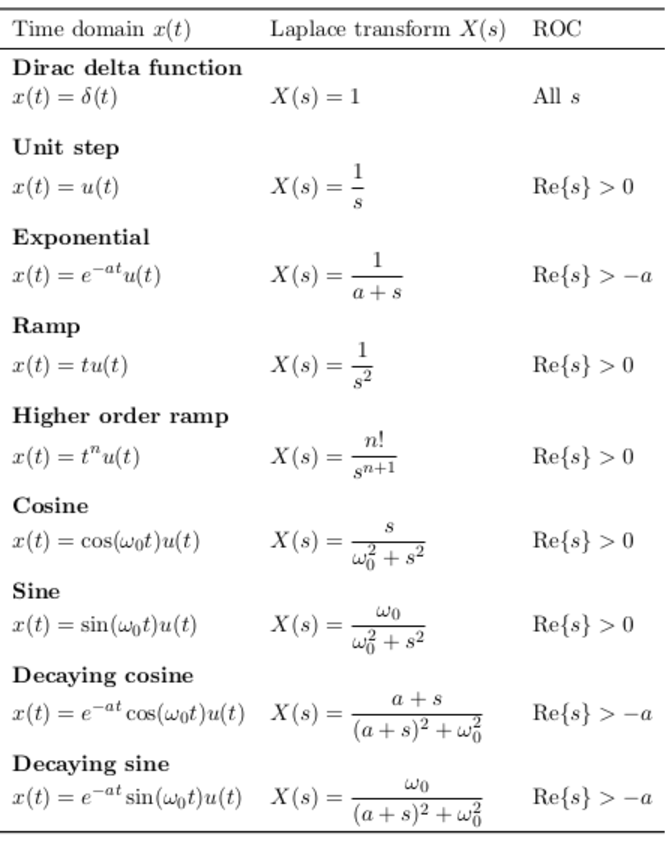
\includegraphics[width=12cm]{image/unilateral-Laplace-transform-pairs.pdf}
    \caption{Unilateral Laplace transform pairs. From \cite{}}
\end{figure}

\subsection{Properties}
\begin{itemize}
    \item \textbf{Linjarity}: 
     $\alpha x_1(t) + \beta x_2(t) \TransformHoriz \alpha X_1(s) + \beta X_2(s)$
    \item \textbf{Time and frequency scaling}: 
    $x(at) \TransformHoriz \frac{1}{a}X(\frac{s}{a})$ for $a>0$
    \item \textbf{Time and frequency shifting}: 
    \begin{itemize}
        \item $x(t-\Delta t) \TransformHoriz X(s)e^{-s\Delta t}$
        \item $x(t)e^{at} \TransformHoriz X(s-a)$
    \end{itemize}
    \item \textbf{Convolution and multiplication}: 
    \begin{itemize}
        \item $x_1(t)*x_2(t) \TransformHoriz X_1(s)X_2(s)$ 
        \item $x_1(t)x_2(t) \TransformHoriz \frac{1}{2\pi j}X_1(s)*X_2(s)$ 
    \end{itemize}
    \item \textbf{Differentiation and integration}: $\frac{d^nx(t)}{dt^n} \TransformHoriz sX(s)-x(t)$ 
    \item \textbf{Initial and final value theorems}: 
    \begin{itemize}
        \item $\lim_{t\to0}x(t) = \lim_{s\to\infty} sX(s)$
        \item $\lim_{t\to\infty}x(t) = \lim_{s\to0} sX(s)$
    \end{itemize}
\end{itemize}


\subsection{Transfer function}

\subsubsection{Solving differential equations}
Can solve Differentiation equations. Use Laplace transforms then do the inverse transform.
The analyzing system is useful to use transform. It is done the same way as for solving differential equations.
This works for all dimensions.

%\begin{exampleblock}{Example: ODE solving with transfer functions}
%TODO
%\end{exampleblock}

\begin{align*}
    H(s) &= \frac{Y(s)}{X(s)}=\frac{s^{M}b_M + s^{M-1}b_{M-1} + \ldots + b_0}{s^{N}b_N + s^{N-1}b_{N-1} + \ldots + a_0} \\
    Y(s) &= H(s)X(s)
\end{align*}

\subsubsection{Transfer functuion and impuslse response}
\begin{align*}
    &h(t) \TransformHoriz H(s) \\
    &H(s) = \int_{0}^{\infty} h(t)e^{-st}dt
\end{align*}

\subsubsection{Transfer functuion and frequency response}
The relationship between the transfer function $H(s)$ and the frequency response 
$H(j\omega)$ of a continues time LTI system is given by 
\begin{align*}
    &H(j\omega) = H(s)|_{j\omega}
\end{align*}

\subsubsection{Poles and Zeros, and Stability}
% In other words, the roots are the points in the s-plane where the polynomials become
%zero: If zi is a root of the numerator polynomial B(s), it must hold that
%B(zi) = 0,
%and if pj is a root of the denominator polynomial A(s), it must hold that
%A(pj) = 0.

\begin{align*}
    H(s) &= K\frac{(s-z_1)(s-z_s)\ldots(s-z_M)}{(s-p_1)(s-p_2)\ldots(s-p_N)} \\
    &\text{where $z_M$ is zeros} \\
    &\text{and $p_N$ is poles}
\end{align*}

The system is proper if $N\geq M$ and strictly proper if $N>M$. 
It is stable if all $p_i<0$.  \newline

If $p_i=0$ then the output will never convert just alternate to infinity (unstable). \newline
\indent If $p_i>0$ then it will increase it's amplitude (unstable). \newline

LTI system is stable if and only if the real part of all of its poles is negative. \newline

\textit{Steady-state} is when amplitude is $A=|H(s)|_{s=j\omega_0}$ and phase $\phi=H(s)_{s=j\omega_0}$ \newline

The poles tells us when the transfer function $H(s)$ becomes a division by zero. 
The zeros meanwhile tells us when then the function is zero. The Pole-Zero Map 
is a display from the top looking down where x is the marked when the expression goes to infinite and
the zero is when the expression is zero.

\begin{exampleblock}{Example: Poles and Zeros}%Example: Poles and Zeros, Stability analysis
Consider a linear, time-invariant system describe ed by the differential equation
\begin{equation*}
    \frac{d^2y(t)}{dt^2} + 6\frac{dy(t)}{dt} + 13y(t) = \frac{dx(t)}{dt} + 2x(t)
\end{equation*}
Assume that all initial conditions are zero.
Determine wether or not the system is stable.

\textbf{Solution}:
Determine the transfer function $H(s)$
\begin{align*}
    &s^2Y(s) +6sY(s) + 13Y(s) = sX(s) + 2X(s) \\
    &Y(s)(s^2+6s+13) = X(s)(s+2) \\
    &\frac{Y(s)}{X(s)} = \frac{s+2}{s^2+6s+13} = H(s)
\end{align*}
we se that the system is proper since the degree of the enumerated is less the denominator

Zeros:
\begin{align*}
    &s+2=0 \\
    &s=-2 \Rightarrow z_1=-2
\end{align*}

Poles:
\begin{align*}
    &s^2+6s+13 = 0 \\
    &s=-\frac{6}{2}\pm\sqrt{3^2-13}=-3\pm\sqrt{-4}=-3\pm 2j \\
    &\Rightarrow p_{1,2} = -3\pm 2j
\end{align*}

There of do we see that both poles are negative, there fore is the system stable.
\end{exampleblock}

\textit{qualitative} impulse response.

\subsection{Bod plot}
Bode plots can relatively easily be constructed by hand, which was
paramount before the computer era for analyzing complex dynamic systems. \newline

Bode plots are a standardized way of plotting a system's frequency response function
and a Bode plot actually consists of two plots: A Bode magnitude plot (or simply
magnitude plot ) and a Bode phase plot (or simply a phase plot). \newline

Asymptote is the line where define the direction of the line.


\begin{equation*}
    |H(j\omega)|_{dB} = 20\log_{10}(|H(jw)|)
\end{equation*}

\subsubsection{Bode Form of Transfer Function}
\begin{align*}
    H(s) &= K \frac{(s-z_1)\ldots(s-z_M)}{s^l(s-p_1)\ldots(s-p_{N-l})} \\
    H(s) &= K_0 \frac{ (\frac{s}{z_1}+1)\ldots((\frac{s}{\omega_{n,i}})^2+2s\frac{\zeta_i}{\omega_{n,i}}+1)\ldots }{ s^l( \frac{s}{p_1}+1) \ldots ((\frac{s}{\omega_{n,j}})^2+2s\frac{\zeta_j}{\omega_{n,j}}+1)\ldots } \\
    K_0 &= K \frac{ \prod_i(-z_i) }{ \prod_i(-p_i) }
\end{align*}
There are $l$ poles in the origin (the term $s^{-l}$). 


\subsubsection{Sketching Bode Plots}
\begin{exampleblock}{Example: ODE solving with transfer functions}
Sketch Bode plots for the following transfer functions.
\begin{equation*}
    H(s) = \frac{s(s+100)}{(s+2)(s+20)}
\end{equation*}

\textbf{Solution:}
First we write the transfer function as in bode normal Form
\begin{align*}
    H(s) &= \frac{s(s+100)}{(s+2)(s+20)} 
     = \frac{100 s(\frac{s}{100}+1)}{2\cdot20(\frac{s}{2}+1)(\frac{s}{20}+1)} \\
    H(j\omega) &= \frac{100 j\omega(\frac{j\omega}{100}+1)}{2\cdot 20(\frac{j\omega}{2}+1)(\frac{j\omega}{20}+1)}
     = \frac{100 j\omega(1+j\frac{\omega}{100})}{2\cdot 20(1+j\frac{\omega}{2})(1+j\frac{\omega}{20})}
\end{align*}

\begin{align*}
    &\lim_{\omega\to 0} H(j\omega) = 0, (-\infty dB) \\
    &\lim_{\omega\to \infty} H(j\omega) = 1, (0 dB)
\end{align*}

We can write the magnitude by adding the factor together
\begin{align*}
    |H(j\omega)|_{dB} &= 20\log_{10}(\frac{100}{2\cdot 20})
    +20\log_{10}(|j\omega|) 
    -20\log_{10}(\big| 1+j\frac{\omega}{2}\big|) \\
    &\;\;\; -20\log_{10}(\big| 1+j\frac{\omega}{20}\big|)
    +20\log_{10}(\big| 1+j\frac{\omega}{100}\big|)
\end{align*}

The phase shift can be done similarly.
\begin{align*}
    &\angle \frac{100}{2\cdot 20} = 0 \\
    &\angle |j\omega| = \frac{\pi}{2} \\
    &\angle \frac{1}{1+j\frac{\omega}{2}} = -\angle 1+j\frac{\omega}{2} =
    \left\{\begin{array}{ll}
      0 \;\;\;\;\;\;\, w=0 \\
      -\frac{\pi}{4} \;\;\; w=2 \\
      -\frac{\pi}{2} \;\;\; w\to\infty
    \end{array}\right. \\
    &\angle \frac{1}{1+j\frac{\omega}{20}} = -\angle 1+j\frac{\omega}{20} =
    \left\{\begin{array}{ll}
      0 \;\;\;\;\;\;\, w=0 \\
      -\frac{\pi}{4} \;\;\; w=20 \\
      -\frac{\pi}{2} \;\;\; w\to\infty
    \end{array}\right. \\
    &\angle 1+j\frac{\omega}{100} = 
    \left\{\begin{array}{ll}
      0 \;\;\;\;\;\;\, w=0 \\
      \frac{\pi}{4} \;\;\; w=100 \\
      \frac{\pi}{2} \;\;\; w\to\infty
    \end{array}\right. 
\end{align*}

Now we can draw the bode plot see figure \ref{fig:bodePlotExample}.
\end{exampleblock}

\begin{figure}[H]
    \centering
    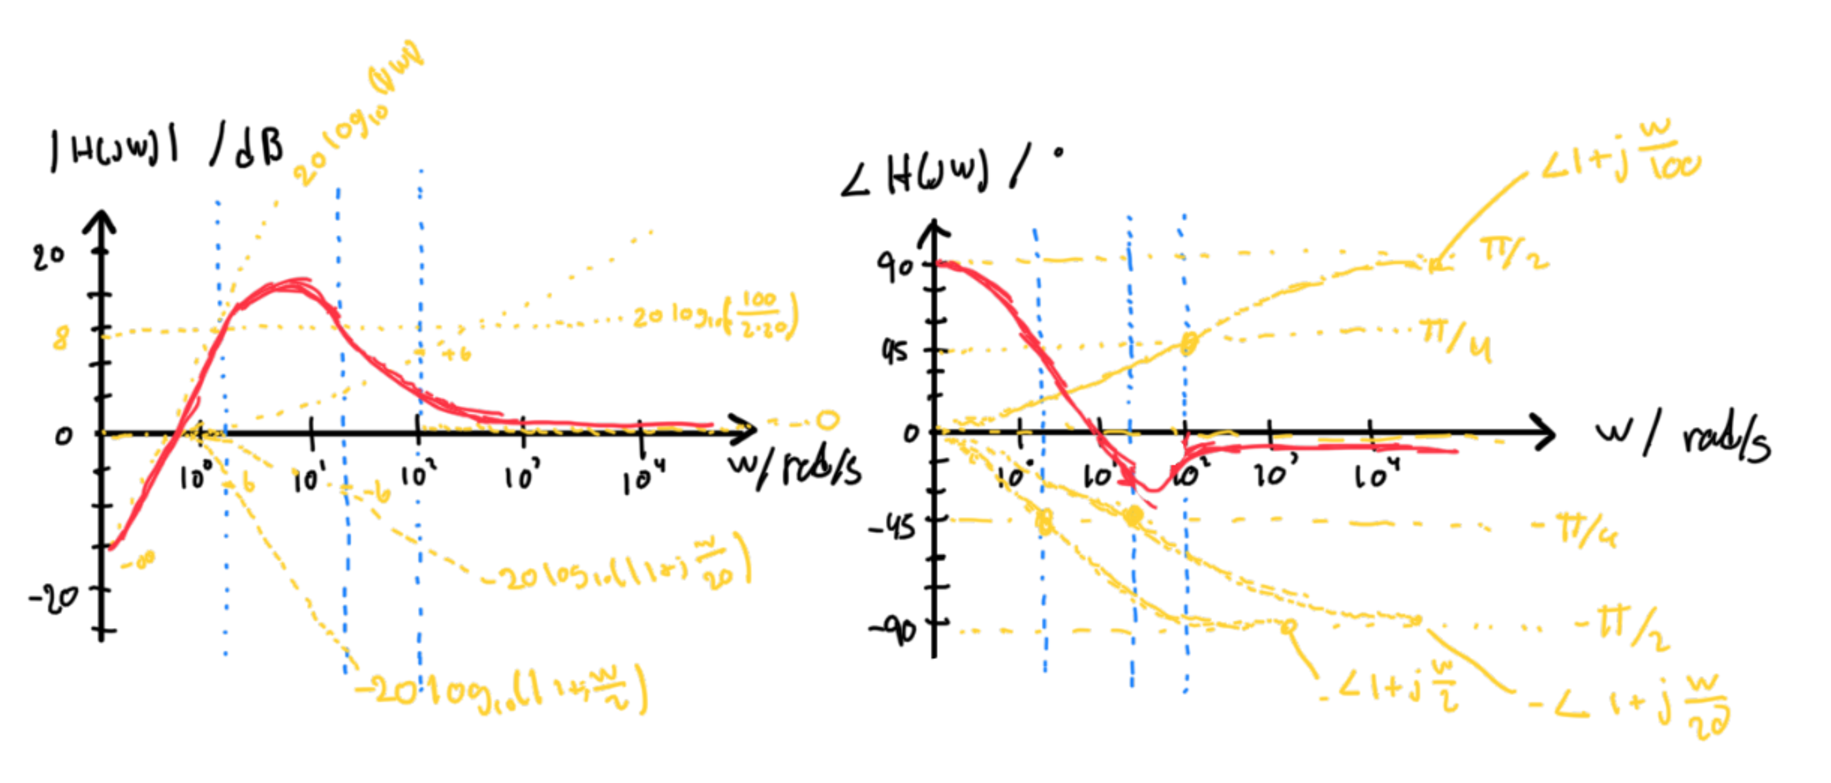
\includegraphics[width=12cm]{image/bode-plot-example.pdf}
    \caption{Bode plot example}
    \label{fig:bodePlotExample}
\end{figure}


%\textbf{Constant}: The gain $K0$ appears as a constant function independent of the frequency
%$\omega$ in the Bode plot. 
%\begin{equation*}
%    |K_0|_{dB} = 20\log(|K_0|)
%\end{equation*}
%
%\textbf{Poles at the origin}:
%Poles in the origin yield the term $(j\omega)^-l$ in the frequency response.
%\begin{equation*}
%    20\log_{10}(|(\omega)^{-l}|) = -20l\log_{10}(\omega)
%\end{equation*}
%
%\textbf{First order term}: A first order term has the form $(\frac{j\omega}{\alpha})^{\pm 1}$
%\textbf{Second order term}:
%\textbf{Phase shift}:

%Bounded input bounded output it is bounded from max and min values.
%proper: n is greater than m, where n is the degree of the numerator m is the degree of the denominator 
%bod plot
%tent plot, determent the frequency response

\section{Filtering theory}
\subsection{Filtering Theory and Ideal Filters}
An ideal filter only contains a \textit{passband} (the frequency range that the signal is not filterd out) 
and the \textit{stopband} (the frequency witch is filtered out)

%Have image of the diffrent types better in videos
%and formulas for each
\begin{itemize}
    \item \textbf{Lowpass filter}:
    $H_{LP}(\omega) = rect\big( \frac{\omega}{2\omega_c} \big)$
    \item \textbf{Highpass filter}:
    $H_{HP}(\omega) = 1-rect\big( \frac{\omega}{2\omega_c} \big)$
    \item \textbf{Bandpass filter}:
    $H_{BP}(\omega) = rect\big( \frac{\omega}{2\omega_{c2}} \big) - rect\big( \frac{\omega}{2\omega_{c1}} \big)$
\end{itemize}
Where $\omega_c$ is the cut-off frequency.

\begin{figure}[H]
    \centering
    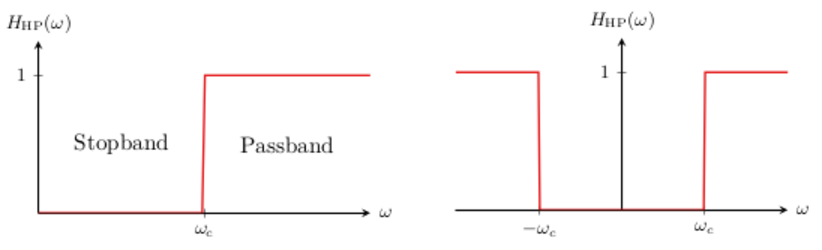
\includegraphics[width=12cm]{image/filter-lp-hp.pdf}
    \caption{Lowpass and Highpass filter. From \cite{}}
    \label{fig:filter-lp-hp}
\end{figure}

\begin{figure}[H]
    \centering
    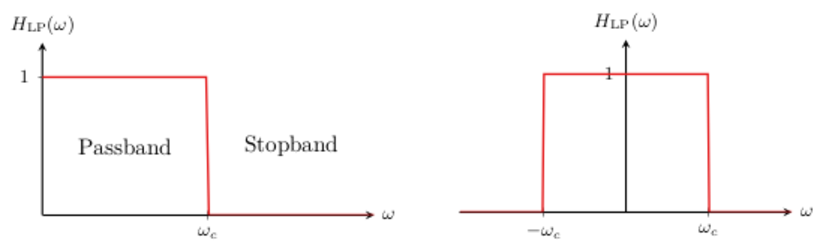
\includegraphics[width=12cm]{image/filter-bp-bs.pdf}
    \caption{Bandpass and Bandstop filter. From \cite{}}
    \label{fig:filter-bp-bs}
\end{figure}


%\delta_p magnitude of frewuency response. (GOOD IMAGE 5.40)

\subsection{Filter Approximations}
Ideal filters can not be implemented there for we use approximations. 

% good images
\begin{figure}[H]
    \centering
    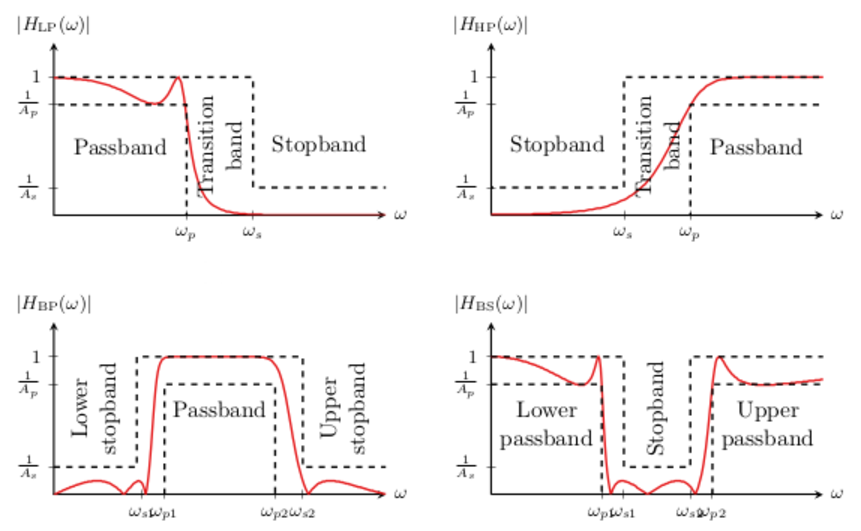
\includegraphics[width=12cm]{image/approximation-spectrum.pdf}
    \caption{approximation-spectrum. From \cite{}}
    \label{fig:approximation-spectrum}
\end{figure}

\begin{multicols}{2}
\begin{itemize}
    \item \textit{passband ripple}: maximum amount of attenuation allowed in the passband.
    \item \textit{passband edge frequency}: the frequency that markes the end of the requirment on the passband ripple
    \item \textit{stopband attenuation}: the minimum attenuation in the stopband
    \item \textit{stopband edge frequency}: the frequency  that marks the start of the requirment on the stopband.
\end{itemize}

\textbf{Cut-off frequency definition}
\begin{equation*}
   |H(\omega_c)| = \frac{1}{\sqrt{2}} \approx 0.707 = -3dB
\end{equation*}


\textit{Roll-off rate} is how quickly the real filter transition between the pass- and stopband.
\begin{equation*}
    R=\frac{d}{d\omega}\log_10(|H(\omega|^2)\Big|_{\omega=\omega_c} = 2\frac{d}{d\omega}\log_10(|H(\omega)|)\Big|_{\omega=\omega_c}
\end{equation*}


\subsubsection{Approximation Types}
\begin{itemize}
    \item \textbf{Butterworth filter}:
    \begin{itemize}
	\item $|H(\omega)| = \dfrac{1}{\sqrt{1+\big(\dfrac{\omega}{\omega_c}\big)^{2N}}}$
	\item $N\geq \dfrac{\log\Big(\sqrt{\dfrac{A_s^2-1}{A_p^2-1}}\Big)}{\log\big(\dfrac{2\pi f_s}{2\pi f_p}\big)}$
    \end{itemize}
    \item \textbf{Chebyshev Type I filters}: % write how to get the N for all
    \begin{itemize}
	\item $|H(\omega)|=\dfrac{1}{\sqrt{1+e^2T_N^2\big(\dfrac{\omega}{\omega_p}\big)}}$
	\item $N\geq \dfrac{arccosh\Big(\sqrt{\dfrac{A_s^2-1}{A_p^2-1}}\Big)}{arccosh\big(\dfrac{2\pi f_s}{2\pi f_p}\big)}$
    \item $T_N=\left\{\begin{array}{ll}
        \cos(N arccos(\omega)) \text{ for } |\omega|\leq 1 \\
        cosh(N arccosh(\omega)) \text{ for } |\omega|> 1 
    \end{array}\right.$
    \end{itemize}
    \item \textbf{Chebyshev Type II filters}:
    \begin{itemize}
	\item $|H(\omega)|
    = \dfrac{1}{\sqrt{1+\big[e^2T_N^2\big(\dfrac{\omega_s}{\omega}\big)\big]^{-1}}} 
    = \sqrt{\dfrac{e^2T_N^2\big(\dfrac{\omega_s}{\omega}\big)}{1+e^2T_N^2\big(\dfrac{\omega_s}{\omega}\big)}}$
	\item $N = $
    \item $A_p = 10^{(\text{passband ripple}/20)}$
    \item $\epsilon = \sqrt{A_p^2-1}$
    \end{itemize}
    \item \textbf{Elliptic filters}:
    \begin{itemize}
	\item $|H(\omega)|=$
	\item $N=$
    \end{itemize}
\end{itemize}

Where $A_p$ is passband attenuation, $A_s$ stopband attenuation. 
$\omega_c$ is cutoff frequency in $rad/s$, $f_c$ is cutoff frequency in $Hz$.
$\omega_s$ is the stopband edge frequency. $\epsilon$ ripple control factor.
$N$ is the order.
\begin{itemize}
	\item $R_p, \; R_s$ (in dB). 
	\item $A_p=10^{R_p/20}$
	\item $A_s=10^{R_s/20}$
\end{itemize}

\href{https://en.wikipedia.org/wiki/Butterworth_filter}{Butterworth}
\href{https://www.semanticscholar.org/paper/Low-pass-filter-approximation-with-evolutionary-Ayten-Vural/447a00e54c1abb6e98ddf243a3de1cba33cd5200/figure/0}{Chebyshev}

% Why looking at the polse? to se ther stablitity
%\textbf{Butterworth filter}
%A spesific type of low pass filter. 
%what is the diffrence between butterworth filter and low pass filter? more efficent since it has a proximations

%two formalised one normalised and the other not.
%exist higer order of butterworth filters

%complex unit sircuil. Complex conjugates are alsasw tha case and debending on the order there are spaced diffrently.
%end pulse.

%cuoff frequency, zero frequency, maximumvalued flat, roll-off filter(Increase N coser to ideal filter)

%There is a formula for N dependeng on what you desigerd. 

%\textbf{Chebyshev Type I filters}
%There is no ribbles for type 1
%\textbf{Chebyshev Type II filters}
%This has zeros

%alternative to butterworth
%chebyshev polynomial. 
%there is a trade-off when designing a chebyshev filters. increasing the riple control factor biger triple.
%if smaller the smaller roll-off, smaller ripple
%if increasing N faster roll-off, more ripples
%if small N slower roll-off, less riples
%%(4.40)
%type 1 and type 2 chebyshev filters

%\textbf{eliptic fulters}
%there is riples in past band and the stop band

\subsubsection{Filter design}
%exampples
\begin{exampleblock}{Example: Filter desing for Butterworth and Chebyshev type 1}
	TODO
\end{exampleblock}

%\textbf{Frequency transfomrmation}
%Transform from low pass to highpass and vise fersa
%low pass to band pass, low pass to band stop.


Realed valued
how to convert from dB to non dB
what is sinc cosh arccosh


\section{Sampling and Reconstruction}
\begin{figure}[H]
    \centering
    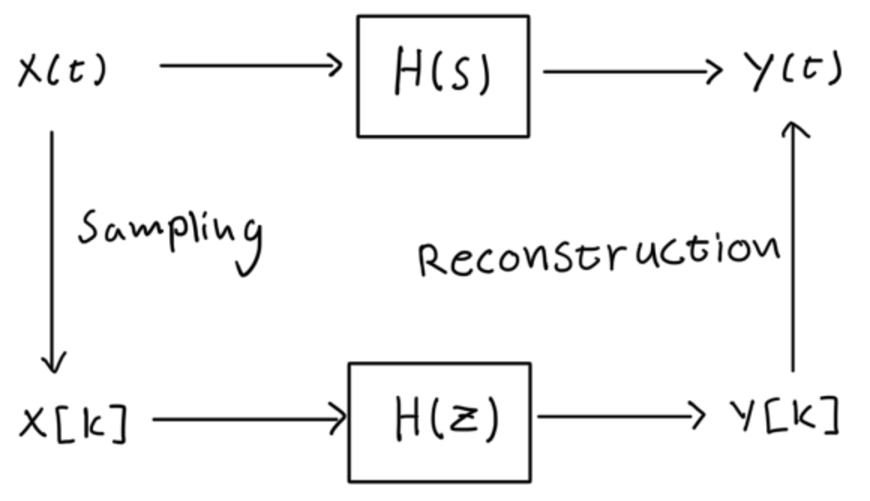
\includegraphics[width=8cm]{image/sampling_and_reconstruction.pdf}
    \caption{Sampling and Reconstruction}
    \label{fig:sampling_and_reconstruction}
\end{figure}

\begin{equation*}
    x[k] \delequal x(k T_s)
\end{equation*}
Where $T_s$ is the time delta for samplening and $k$ is a integer. \newline

We can do sampling in the time domain and in the frequncy domain. 
We us a sampling signal with is a diract delta function with is multiplied with 
the input signal in the time domain.

\noindent\textit{Bandlimiting} is the limiting of signal's frequency domaian representation.

\subsection{Sampling}
The sampling frequncy $\omega_s$ is equal to the higest frerquency $\omega_b$ (b stands for bandwidth)
time two.
\begin{equation*}
    \omega_s > 2\omega_b    
\end{equation*}

\subsubsection{Nyquist-Shannon Sampling Theorem}
The creteria for sampling to work as inteded.
\begin{align*}
    &\omega_s =\frac{2\pi}{T_s} \\
    &\omega_s > 2\omega_b \\
    &f_s > 2f_c \text{ or } T_s < \frac{1}{2f_b} \\
    &\omega_N = \frac{\omega_s}{2}
\end{align*}


In order to get the sampled signal we need to do the following.
\begin{equation*}
    x[k]=x(kT_s)=x_s(t)=x(t)s(t)
\end{equation*}

The \textit{impulse train} ($s(t)$) consisting of $T_s$-periodc Dirac delta functions.
\begin{equation*}
    s(t) = \sum_{k=-\infty}^{\infty} \delta(t-kT_s)
\end{equation*}

Impulse train in the frequency domain yields:
\begin{equation*}
    S(\omega) = \mathcal{F}\{s(t)\} = \frac{2\pi}{T} \sum_{m=-\infty}^{\infty} \delta(\omega-m\omega_s)
\end{equation*}
And the output then becomes:
\begin{equation*}
    X_s(\omega) = \frac{1}{2\pi}X(\omega) * S(\omega)
\end{equation*}

\textit{Oversampling} is the result of choosing a sampling frequency $\omega_s$ larger then the Nyquist frequncy $\omega_N$,
but still smaller then the maximum frequency $\omega_b$.

\begin{figure}[H]
   \centering
   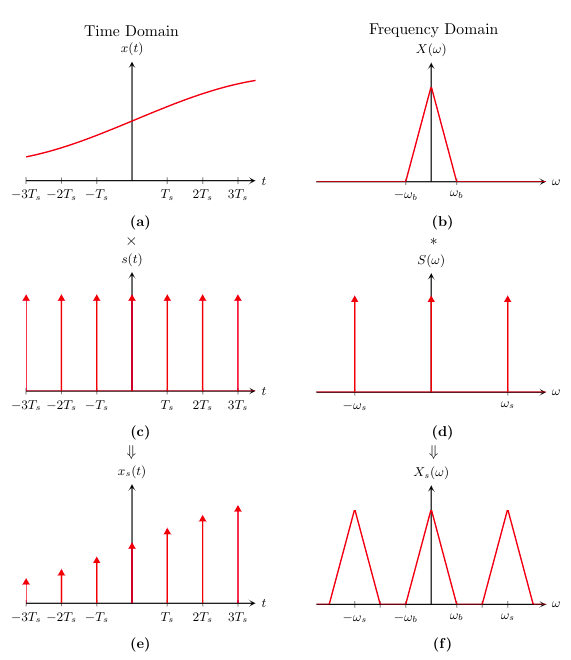
\includegraphics[width=8cm]{image/sampling_graphs.png} 
   \caption{Sampling Graphs. From \cite{st}}
   \label{fig:sampling_graphs}
\end{figure}


\subsubsection{Aliasing and Anti-Aliasing}
Aliasing accures when 
\begin{equation*}
    \omega_s < 2\omega_b
\end{equation*}

\begin{figure}[H]
    \centering
    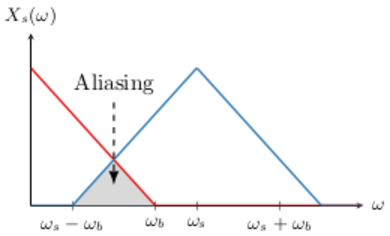
\includegraphics[width=8cm]{image/aliasing.pdf}
    \caption{Aliasing. From \cite{st}}
    \label{fig:aliasing}
\end{figure}
If there is overlap, one can not recover the signal and are therfore useless.

A anti-aliasing filter is plased before the annalog to digital conversion (ADC).
Idealy would the filter block above the maximum signal frequncy $\omega_b$ but this 
it is not possible to implement such a filter witch garantes it and there for will 
there be a small amount of aliasing leaking through.


\subsection{Reconstruction}
A ideal low pass filter can be used for reconstruction, since one can get the signals frequencies.
The filter is a rect in the frequency domain and there for a sinc in the time domain.
\begin{figure}[H]
    \centering
    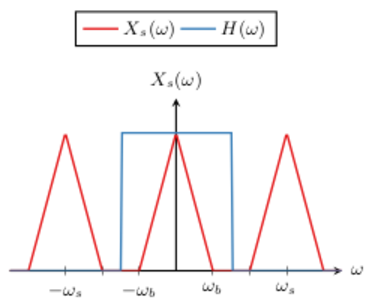
\includegraphics[width=8cm]{image/ideal_reconstruction.pdf}
    \caption{Ideal reconstruction. From \cite{st}}
    \label{fig:ideal_reconstcion}
\end{figure}

\textit{Zero-order hold} (ZOH) is used to keep the output constant for the sampling period.
After ZOH a smothing filter is used.

\begin{align*}
    x_{zoh}(t) &= x_s(t)*rect\Big(\frac{t-T_s/2}{T_s}\Big) \\
    X_{zoh}(\omega) &= X_s(\omega)T_s sinc\Big(\frac{\omega T}{2\pi}\Big)e^{j\omega\frac{T_s}{2}}
\end{align*}
\end{multicols}
\raggedcolumns


\subsection{Quantization}
The amount of lavels witch the digital signal can hold.

\begin{figure}[H]
    \centering
    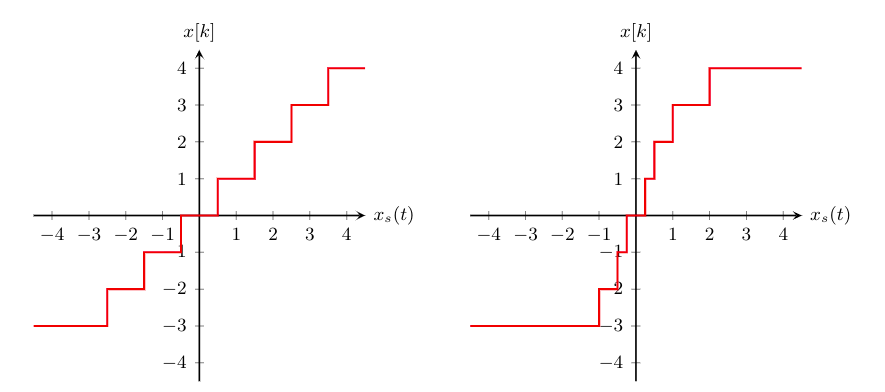
\includegraphics[width=12cm]{image/quantization.png}
    \caption{Two 3 bit quantizers ($L=2^3=8$). (a) uniform quantizer (b) non-uniform quantizer. From \cite{}}
    \label{fig:quantization}
\end{figure}


\section{Discrete time signals and systems}
Discrete time signals in only define on a valid integer $k$. Therefore can we not have 
a stem one $0.5$ for instance.

$K_0$ is the descrete time period. Therefore is the following true for periodc dicrete time signals
\begin{equation*}
   x[k] = x[x+K_0]
\end{equation*}

also, the continus time period can be derived
\begin{equation*}
    K_0T_s = T_0
\end{equation*}

\begin{exampleblock}{Example: Determine how many samples is needed}
    If you were to calculate the DFT using K samples of the signal without zero padding,
    how many samples do you need when the signal is 
    \begin{equation*}
        x[k] = 0.5\cos\left(2\frac{2\pi}{10}k\right) + \cos\left(3\frac{3\pi}{10}k\right) \text{?}
    \end{equation*}

    We know $\frac{\omega_s}{K}\leq \Delta\omega$ where $x_1(t)=\cos\left(\omega_1 t\right)$ and $x_2(t)=\cos((\omega_1 +\Delta\omega)t)$

    \begin{align*}    
        &\Delta\Omega = \frac{2\pi}{K}, \;\; \Delta\Omega = 3\frac{2\pi}{10} - 2\frac{2\pi}{10} = \frac{2\pi}{10}  \\
        &\frac{2\pi}{K} = \frac{2\pi}{10} \Rightarrow K = 10
    \end{align*}
    Hence the we need 10 samples.
\end{exampleblock}


\subsection{Discrete Time Signals}
\subsubsection{Elementary Discrete Time Signals}
\begin{itemize}
    \item \textbf{Sine and cosine signals}: 
    \begin{itemize}
        \item $x[k] = A\sin(\Omega_0 k + \varphi)$
        \item $x[k] = A\cos(\Omega_0 k + \varphi)$
    \end{itemize}
    \item \textbf{Unit impulse}: 
    \begin{itemize}
        \item $\delta[k] = \left\{\begin{array}{ll} 1 & \text{ for } k=0 \\ 0 & \text{ for } k \neq 0 \end{array}\right.$
    \end{itemize}
    \item \textbf{Rectangular pulse}: 
    \begin{itemize}
        \item $rect\Big[\frac{k}{2N+1}\Big] = \left\{\begin{array}{ll} 1 & \text{ for } |k| \neq N \\ 0 & \text{ for } |k| > N \end{array}\right.$
    \end{itemize}
    \item \textbf{Unit step}: 
    \begin{itemize}
        \item $u[k] = \left\{\begin{array}{ll} 0 & \text{ for } k < 0 \\ 1 & \text{ for } k \geq 0 \end{array}\right.$
    \end{itemize}
    \item \textbf{Sinc}: 
    \begin{itemize}
        \item $sinc\Big[\frac{k}{K_0}\Big] = \frac{\sin\big(\pi\frac{k}{K_0}\big)}{\pi\frac{k}{K_0}}$
    \end{itemize}
\end{itemize}


\subsubsection{Discrete Time Signal Properties}
\begin{itemize}
    \item \textbf{Periodic signals}: $x[k]=x[k+K_0]$
    \item \textbf{Causal signals}: $x[k]=0$ for $k<0$
    \item \textbf{Energy and power signals}: (can never be both)
    \begin{itemize}
        \item $E=\sum_{k=-\infty}^{\infty} |x[k]|^2$ where $0<E<\infty$
        \item $P=\lim_{K\to\infty}\frac{1}{K+1}\sum_{k=-K/2}^{K/2} |x[k]|^2$ for aperiodic signals
        \item $P=\frac{1}{K_0}\sum_{k=0}^{K_0-1} |x[k]|^2$ for periodic signals
    \end{itemize}
\end{itemize}

$\Omega_0 = \frac{2\pi}{K_0}$

\subsection{Time Domain Analysis of Discrete Time Systems}
\subsubsection{Impulse Response}
\begin{align*}
    \delta[k] &\mapsto h[k] \\
    \alpha\delta[k-k_0] &\mapsto \alpha h[k-k_0]
\end{align*}

\subsubsection{Convolution Sum}
input output relationship for descrite time (definition)
\begin{align*}
    y[k] &= \sum_{m=-\infty}^{\infty} h[k]x[k-m] = h[k]*x[k] \\
    y[k] &= \sum_{m=0}^{\infty} h[k]x[k-m] \text{ for casual systems}
\end{align*}

\begin{figure}[H]
    \centering
    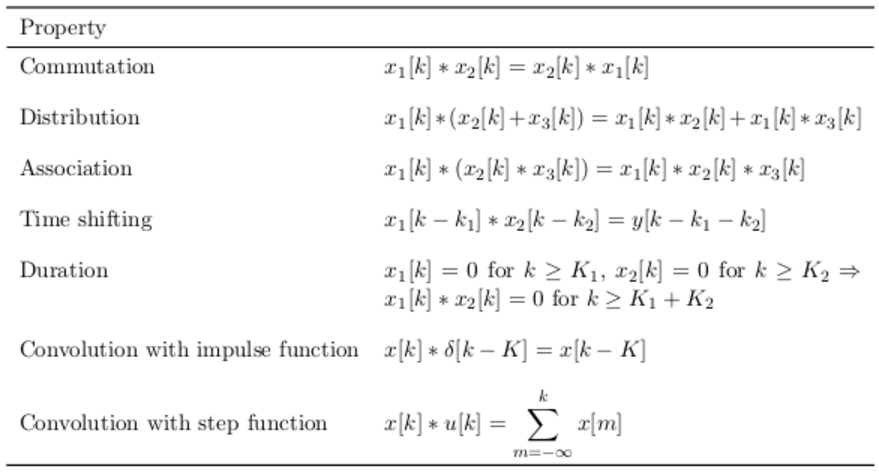
\includegraphics[width=12cm]{image/properties_of_the_discreate_time_convolution_sum.pdf}
    \caption{Properties of the discrete time convolution sum. From \cite{}}
    \label{fig:properties_of_the_discreate_time_convolution_sum}
\end{figure}


\section{Discrete Time Fourier Analysis}
\subsection{Discrete Time Fourier Series and Transform}
\subsubsection{Definition and Properties}
\textbf{Definition of Discrete time Fourier transform (DTFT)}
\begin{align*}
    x[k] &= \sum_{n=0}^{K_0-1} \\
    c_n  &= \frac{1}{K_0}\sum_{k=0}^{K_0-1} x[k]e^{-jn\Omega_0k}
\end{align*}

Fourier transform for sampled continous tims signals:
\begin{equation*}
    X(\omega) 
    = \int_{-\infty}^{\infty}x(t) \sum_{k=-\infty}^{\infty} \delta(t-kT_s)e^{-j\omega t}dt
    = \sum_{k=-\infty}^{\infty} x(kT_s)e^{-j\omega kT_s}
\end{equation*}

The frequency can be expression:
\begin{equation*}
    \Omega = \frac{2\pi}{K} \;\; \text{ witch is similar to } \omega=\frac{2\pi}{T}
\end{equation*}

\textit{Normalized frequency}.
\begin{equation*}
    \Omega = \omega T_s = 2\pi\frac{f}{f_s}
\end{equation*}

Mapping frequencies:
\begin{align*}
    \Omega &= 2\pi \Leftrightarrow \omega = \omega_s \\
    \Omega &= \pi \Leftrightarrow \omega = \frac{\omega_s}{2} = \omega_N
\end{align*}

Sampling feqeuency.
\begin{equation*}
    X(\Omega) = \sum_{k=-\infty}^{\infty} x[k]e^{-j\Omega k}
\end{equation*}

\textbf{Definition of Discrete time Fourier transform}
\begin{align*}
    X(\Omega) &= \sum_{k=-\infty}^{\infty} x[k]e^{-j\Omega k} \\
    x[k] &= \frac{1}{2\pi}\int_0^{2\pi} X(\Omega)e^{j\Omega k} d\Omega
\end{align*}

Transfor pair and the important property that the fourier transform is alwase 
$2\pi$ for discrete time.
\begin{align*}
    x[k] &\TransformHoriz X(\Omega) \\
    X(\Omega) &= X(\Omega + 2\pi)
\end{align*}

\begin{figure}[H]
    \centering
    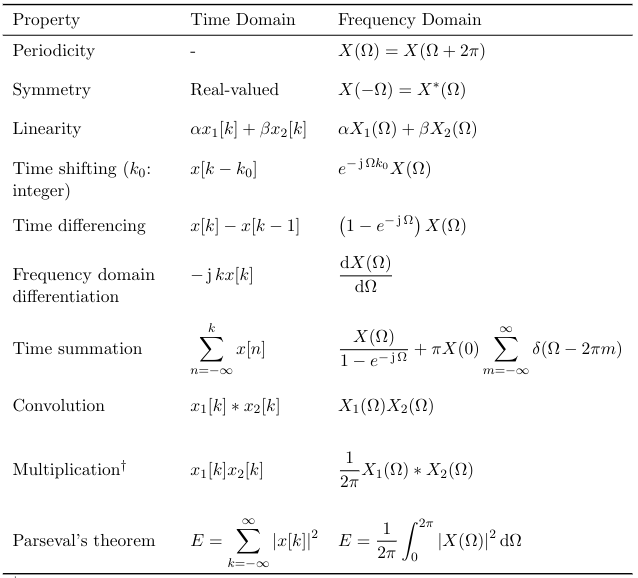
\includegraphics[width=12cm]{image/properties_discrete_time_fourier_transform.png}
    \caption{Properties of the discrete time fourier transform. From \cite{}}
    \label{fig:properties_of_the_discrete_time_fourier_transform}
\end{figure}

% series
% simular to continous time
% geometrik progression is used to derivit D_n

% transform
% magnitude spectrum can determin what type of filter. Only under pi is of intreset

\textit{Hermitian symmetry}: $X(-\omega)=X^*(\omega)$ for realed valued $x[k]$

\subsubsection{Frequency Domain Analysis of Discrete Time Systems}
\begin{align*}
    y[k] &= h[k]*x[k] \\
    x_1[k]*x_2[k] &\TransformHoriz  X_1(\Omega)X_2(\Omega) \\
    Y(\Omega) &= H(\Omega)X(\Omega) \\
    H(\Omega) &= \sum_{k=-\infty}^{\infty} h[k]e^{-j\Omega k}
\end{align*}

% we have desscused four 4 tools for fourier analasys, ctfs, ctft, dtfs, dtfs

\subsection{Discrete Fourier Transform}
With DFT we can determine the spectrum without nowing the signal type
of input signals $x[k]$.

\subsubsection{Definition}
\begin{align*}
    X(l) &= \sum_{k=0}^{K-1} x[k]e^{-jlk\frac{2\pi}{K}} \\
    x[k] &= \frac{1}{K}\sum_{l=0}^{K-1}X[l]e^{jlk\frac{2\pi}{K}}
\end{align*}

Where $L$ is the \textit{Frequency bins}

\begin{figure}[H]
    \centering
    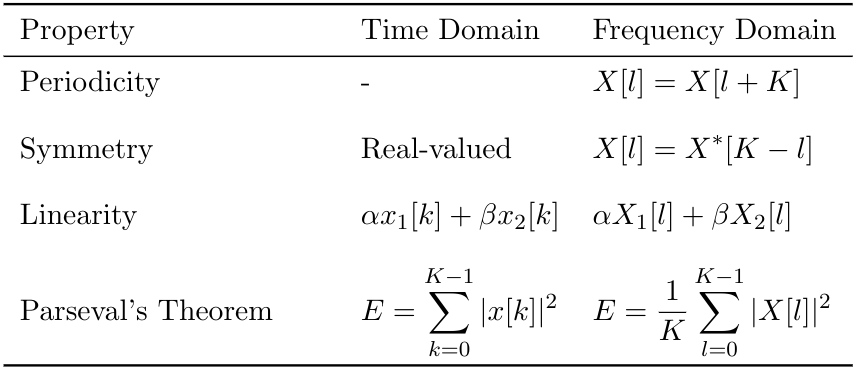
\includegraphics[width=12cm]{image/properties_of_the_dft.png}
    \caption{Properties of the discrete time Fourier transform. From \cite{st}}
    \label{fig:properties_of_the_dft}
\end{figure}


% 3 addoptations gives us the deffinition
\subsubsection{Graphical Interpretation of the DFT}
Calculating the DFT of a sampled continous time signal consists fo the following three steps:
\begin{enumerate}
    \item \textbf{Time domain sampling}. The convolution of $X(\omega)$ and $S(\omega)$
    in the frequency domain, resulting in a spectrum for the sampled signal $x_s(t)$ with 
    $\omega_s$-periodic specrtum with frequency-shift copies of $X(\omega)$. 
    \item \textbf{Time limited}. Windowed signal $x_{sw}(t)=x_s(t)w(t)$, thus the 
    Fourier transform is the convolution between the sampled signal's Fourier transform $X_s(\omega)$
    and $W(\omega)$ (a sinc function). witch yields the spectrum $X_{sw}(\omega)$
    \item \textbf{Frequency domain sampling}. Sampling the frequency domain with a sampling interval of $\frac{\omega_s}{L}$
    This is a multiplication of the sampled signal in time domain and the window signal $x_{sw}(t)$
    with an impulse train in the frequency domain.
\end{enumerate}

% Frequency sampling 
% idealy you have N=M meaning you inly have one window witch you repete, It is dd for each peak in the frequency domain.

\subsubsection{Relationship to the Continuous and Discrete Time Fourier Transforms}
Discrete Fourier Transform (DFT) and dicreate time Fourier Transform (DTFT) are not the
same, however there are similar and there realation is
\begin{equation*}
    X(\Omega)|_{\Omega=l\frac{2\pi}{L}}=X[l]
\end{equation*}
Also DFT is non-zero.

For aperiodic CTFT can be approximated as 
\begin{equation*}
    X(\omega)|_{\omega=l\frac{\omega_s}{L}} \approx T_sX[l]
\end{equation*}
if the continous time signal is limited to interval $0,\ldots,(K-1)T_s$ \newline

In other words $\Omega_l=l\frac{2\pi}{L}$, $\omega_l=l\frac{\omega_s}{L}$,
$f_l=l\frac{f_s}{L}$.

\subsubsection{Zero-Padding, Graphical Resolution, and Spectral Resolution}
\begin{itemize}
    \item \textit{Zero-Padding} is when calculating the DFT for $L>K$.
    \item \textit{Graphical resolution} is the appearance of the spectrum plot.
    \item \textit{Spectral resolution} is the resolution which determines how accurate the calculated Fourier transform is.
\end{itemize}


\subsubsection{Windowing}
\begin{itemize}
    \item \textbf{Rectangular window}: Standard window. Most narrow mainlobe but the strongest sidelobes.
    \item \textbf{Bartlett and triangle windows}: smaller sidelobes then rectangular window but wither mainlobe.
    \item \textbf{Hamming window}: Smother transistions leades to smaller sidelobes and hamming window is the smothers and
    there for the smallest sidelobes.
\end{itemize}

Windowing causes \textit{smering} (wide sidelobes) and \textit{leakage} (new specral content with sidelobes).

\subsubsection{Fast Fourier Transform (FFT)}
One of the most important algorithems ever. It is used for deterimn the fourier transform
of a discrete signal. 
FFT is an efficent way of implementing DFT when $K=2^M$, from $O(K^2)$ to $O(K\log_2(K))$. 
Since the standard way of calculating the fourier transform giledes a matrix multiplication
with $K\times K$, therefore the time complexity is $O(K^2)$. (the matrix is DFT).
There exist symitry in the DFT and other redundent properties, therefore we can optimase 
it. FFT is a optimasiation with split odds and evense into sepreate colums and then multiple
with a diaginal matrix times another matrix.


The \textit{twiddle factor}
\begin{equation*}
    W_K = e^{-j\frac{2\pi}{K}}
\end{equation*}

\begin{align*}
    X[l] &= \sum_{k=0}^{\frac{K}{2}-1}x_1[2k]W_K^{lk} + W_K^{l} \sum_{k=0}^{\frac{K}{2}-1}x[2k+1]W_K^{lk}  \\
    &= X_1[l] + W_k^l X_2[l]
\end{align*}


\section{z-transform}
\subsection{Definition and Properties}
\subsubsection{Definition}
% definition 9.1
% table 9.1
The discrete time Fourier transform for causal signal can be expressed as
\begin{equation*}
    X(\Omega) = \sum_{k=0}^{\infty}x[k]r^{-k}e^{-j\Omega k}
\end{equation*}
where $r^{-k}$ is a decaying exponential function with is used to scale $x[k]$.
The z-transform can then be derived for $z=re^{j\Omega}$.
\begin{align*}
    x[k] &\TransformHoriz X(z) \\
    X(z) &= \sum_{k=0}^{\infty} x[k]z^{-k} \\
    x[k] &= \frac{1}{2\pi j} \oint X(z)z^{k-1}dz
\end{align*}

\begin{figure}[H]
    \centering
    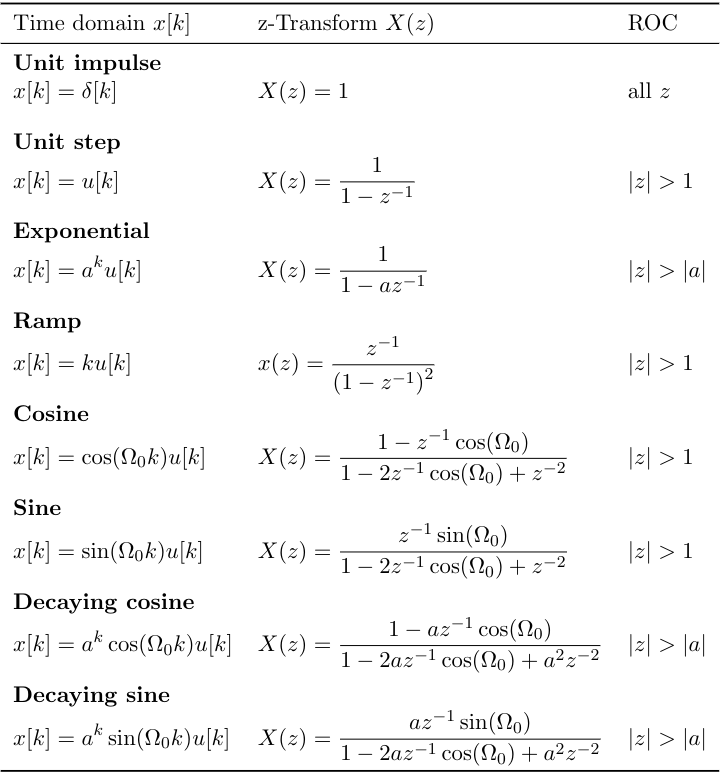
\includegraphics[width=11cm]{image/z-transform_pairs.png}
    \caption{z-transform pairs. From \cite{st}}
    \label{fig:z-transform_pairs}
\end{figure}


\subsubsection{Properties}
% table 9.2
\begin{figure}[H]
    \centering
    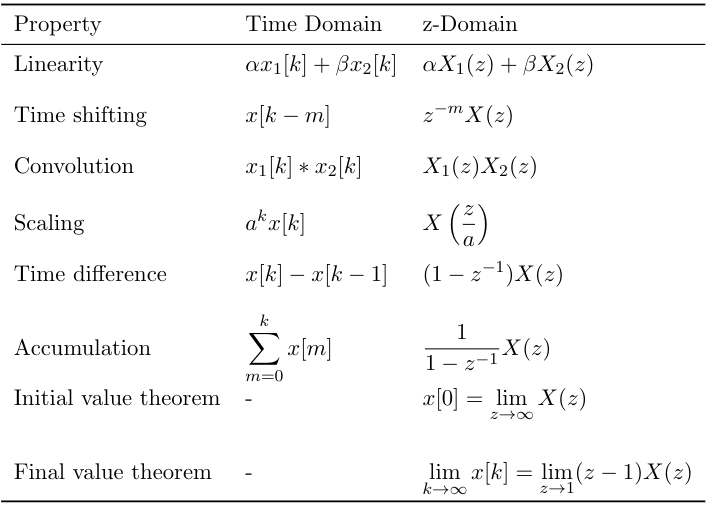
\includegraphics[width=12cm]{image/properties_z-transform.png}
    \caption{properties z-transform. From \cite{st}}
    \label{fig:properties_z-transform}
\end{figure}

%\begin{itemize}
%    \item Liniearity:
%    \item Time shifting:
%    \item Convolution and multiplication:
%\end{itemize}

\subsection{Transfer Function}
\subsubsection{Difference Equations and Transfer Functions}
Input output relationship, is expressed as \textit{difference equations} (recursive)
Somtimes the difference equation are given as looking at $N$ steps into 
the future, in that case the easies approtch is to shifting of diference equations.

\textbf{Definition: Transfer function of discrete time LTI systems}
\begin{align*}
    y[k]+a_1y[k-1]+\ldots+a_N y[k-N] &= b_0 x[k]+b_1 x[k-1]+\ldots+b_M x[k-M] \\ 
    H(z) = \frac{Y(z)}{X(z)} &= \frac{b_0+b_1z^{-1}+\ldots+b_mz^{-M}}{1+a_1z^{-1}+\ldots+a_Nz^{-N}} \\
    Y(z) &= H(z)X(z)
\end{align*}


\subsubsection{Transfer Function and Impulse Response}
% deffinition 9.3
\textbf{Definition: Relationship between the discrete time impulse response and transfrer function}
\begin{align*}
    h[k] &\TransformHoriz H(z) \\
    H(z) &= \sum_{k=0}^{\infty} h[k]z^{-k}
\end{align*}

\subsubsection{Transfer Function and Frequency Response}
% 2\pi periodicfrom \Omega. We get the following deffinion
\textbf{Definition: Relationship between the discrete time transfer function and the frequncy reponse}
\begin{equation*}
    H(\Omega)=H(e^{j\Omega}) = H(z)|_{z=e^{j\Omega}}
\end{equation*}
if the impulse responce is casual, $z=e^{j\omega}$ and the DTFT converges.

\subsubsection{Poles and Zeros, and Stability}
% similar to laplace transform 
Similarly to the laplace transform we can derive the poles and zeros from the tranfer function.
\textbf{Definition: Pole-zero form of the fiscrete time transfer function}
\begin{align*}
    H(z) &= \frac{B(z)}{A(z)} = \frac{b_0+b_1z^{-1}+\ldots+b_mz^{-M}}{1+a_1z^{-1}+\ldots+a_Nz^{-N}} \\
    H(z) &= b_0z^{N-m}\frac{(z-z_1)(z-z_2)\ldots(z-z_M)}{(z-p_1)(z-p_2)\ldots(z-p_N)}
\end{align*}

\textbf{Spectrum behavior for diffrent pole and zero positions}
If the pole is inside the circle it will create a top wich dose not go to 
infiniy. It will however have a higher top the close it is to the circle.

Zeros will have the oposite affect, creating a dip. The closer the the
circle the futher down the dip will reach.

\textbf{Stabiltity}
\begin{figure}[H]
   \centering
   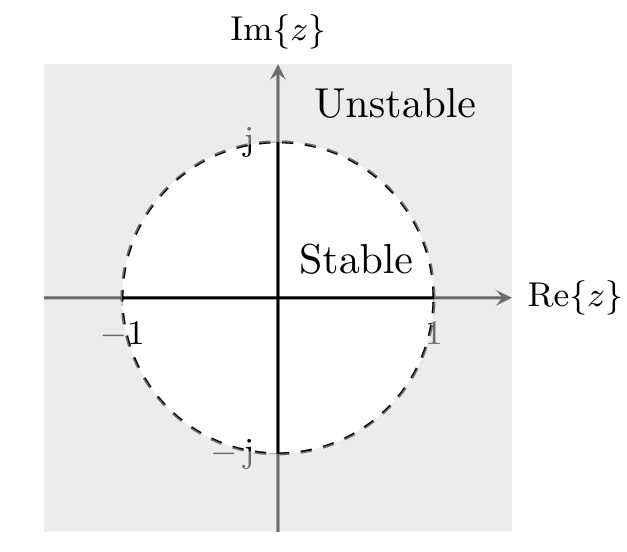
\includegraphics[width=12cm]{image/stability_z-transform.png} 
   \caption{Stability for z-transforms. From \cite{st}}
   \label{fig:stability_z-transform}
\end{figure}

\begin{exampleblock}{Example: stability casual and frequency responce} %{Example: Stability, Casual and Frequency responce}
    What is the systems frequency response and approximate it graphically? Also determin if the system is 
    stable and casual. 
    \begin{equation*}
        y[k+2]+5y[k+1]+0.1y[k] = x[k+1]
    \end{equation*}

    We can see that the the output only depends on previus values there for 
    it can be casual.

    First we determin the systems transfer function
    \begin{align*}
        &z^2Y(z)+5zY(z)+0.1 = zX(z) \;\; \text{ -(Time shifting property)} \\
        &Y(z)(z^2+5z+0.1) = zX(z) \\
        &\frac{Y(z)}{X(z)} = \frac{z}{z^2+5z+0.1} = H(z) \;\; \text{ -(Witch is the tranfer function)}
    \end{align*}

    Next we determin the the poles to se if there are inside the complex unit circle, 
    inorder to determin the stablitity.
    \begin{align*}
        &z^2+5z+0.1 = 0 \\
        &z=\frac{-5}{2}\pm\sqrt{\frac{5^2}{2^2}-0.1}=\frac{-5}{2}\pm\frac{\sqrt{24.6}}{2} \;\; \text{ -(pq-formula)}\\
        &p_1\approx-0.0201, \; p_2\approx-5
    \end{align*}
    Since $|p_2|>1$ is the system not stable.

    Determine the frequency responce
    \begin{equation*}
        H(\Omega) = H(z)|_{z=e^{j\Omega}} = \frac{e^{j\Omega}}{e^{2j\Omega} + 5e^{j\Omega} + 0.1}
    \end{equation*}

    Calculating some points to be able to approximate the graph:
    \begin{align*}
        &|H(\Omega)|_{\Omega=2\pi}| = |H(\Omega)|_{\Omega=0}| = |\frac{e^0}{e^0+5e^0+0.1}| \approx 0.16 \;\; \text{ -($2\pi$-periodic)}\\
        &|H(\Omega)|_{\Omega=3\pi/2}| = |H(\Omega)|_{\Omega=\pi/2}| = |\frac{e^{\pi/2}}{e^{\pi}+5e^{\pi/2}+0.1}| = |\frac{-j}{-1+5(-j)+0.1}| \approx 2 \\
        &|H(\Omega)|_{\Omega=\pi}| = |\frac{e^{\pi}}{e^{2\pi}+5e^{\pi}+0.1}| = |\frac{-1}{1+5(-1)+0.1}| \approx 0.26
    \end{align*}
\end{exampleblock}


\section{Digital Filters}
\subsection{Introduction}
\subsubsection{Background}
\subsubsection{Continous Time Requirements and Digital Filters}
% descrete time frequncy (normalized)
% converting stop band and pass band frequnacy to normalized frequency.

\subsubsection{Digital Filters and LTI Systems}
% z transfer function

\subsection{Finite Impulse Response Filters}
\subsubsection{Definition and Properties}
% deffinition
% H(z)
% all poles is at the origin therfore alwase stable

\textit{Filter taps} are the coefficients $b_n$. Thus, an Nth order filter 
has $N+1$ filter taps (starts from $0$ and ends at $N$)

FIR Filters are allwase stable since it dose not have any poles only zeros.
\subsubsection{FIR Filter Design}
% windowing and Parks-McClellan (de-facto standard for FIR filter design)
\begin{figure}[H]
   \centering
   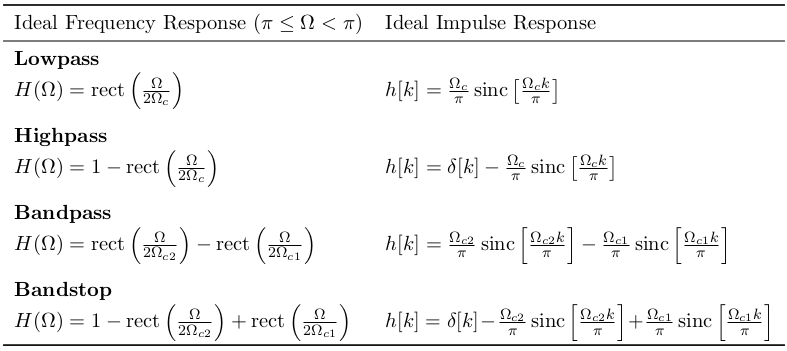
\includegraphics[width=8cm]{image/descrete_time_filter_frequncy_impulse_respons.png} 
   \caption{Descrete time filter frequency responce and their impulse responses}
   \label{fig:descrete_time_filter_frequncy_impulse_respons}
\end{figure}
\textbf{Windowing}
% How windowing filter can be expresed

\textbf{Parks-McClellan}
% The optimal way since it maximise the rippling for pass band and stop band to minimize the order 
% optimization problem

\subsection{Infinite Impulse Response Filters}
\subsubsection{Definition and Properties}
% Output equation
% impulse response

\subsubsection{IIR Filter Design Using the Bilinear Transform}
IIR filter design methods can be divided into two types:
\begin{enumerate}
    \item Indirect methods that are based on converting continuous time filters to discrete time
    \item Direct methods that directly design digital IIR filters in the discrete time domain.
\end{enumerate}

% Direct method: we plase the zeros and poles to get the desired filter (pole zero placment)
% optimization teknic, we select some points on the spectrum that create the desired behavior

%Laplace domain to z domaian

Requirements
\begin{enumerate}
    \item Filter requirement specification (passband and stopband edge frequencies, passband ripple, stopband attenuation);
    \item Design of the analog filter transfer function H(s) (see Chapter 5);
    \item Approximation of the analog filter transfer function using the bilinear transform.
\end{enumerate}

%example

\subsubsection{Filter Coefficient Quantization and Stability}
There could stabile in theroy but unstable in practice. Since the computer may have to 
round the number in a way witch makes the system unstable.

% second order section is a way of spliting a complex filter in to second order filters


\section{How it is connected}
\begin{tabular}{|m{2cm}|m{3cm}|m{4cm}|m{6cm}|}
    \hline
    Consept & Continous signals $x(t)$ & Discreate signals $x[k]$ & Description \\
    \hline
    \hline
    Impulse reponse & $\delta(t) \mapsto h(t)$ & $\delta[k] \mapsto h[k]$ & Is used to determin the output of the system, since the output is $y[k]=h[k]*x[k]$ \\
    \hline
    Frequency reponse & $H(\omega)$ & $H(\Omega)$ with period $2\pi$ & Is the equvilant to the impulse responce in the frequency domain. \\
    \hline
    Signal's spectrum & $X(\omega)$ & $X(\Omega)$ & Is used to view the spectrum where one can se what frequencies dominates \\
    \hline
    Transfer function & $H(s)$ (Laplace) & $H(z)$ (z-transform) & Laplace and z-transform are use to annalyse a system, with polse and zeros. \\
    \hline
    Discrete Fourier transform & - & $X[l]$ & FFT is an algorith to compute the DFT, it turns the samples (wich become a vector) and convert it to a there frequency componetnts. We can not allwase use the DTFT since it requires knoladge of the full signal, not just finite set of samples. \\
    \hline
    Spectrum from DFT calculation & - & $X(f_l)$ with period $f_s$ (???$X(f)$) & We can not alwase determin the signals spectrum analyticly therfore we can approximate it by using the DFT \\
    \hline
\end{tabular}
\textbf{Note:} The fourier tranforms are $X(\omega)$ for Continous tme, $X(\Omega)$ for discreate time and 
$X[l]$ for discreate (NO TIME).  

\begin{figure}[H]
   \centering
   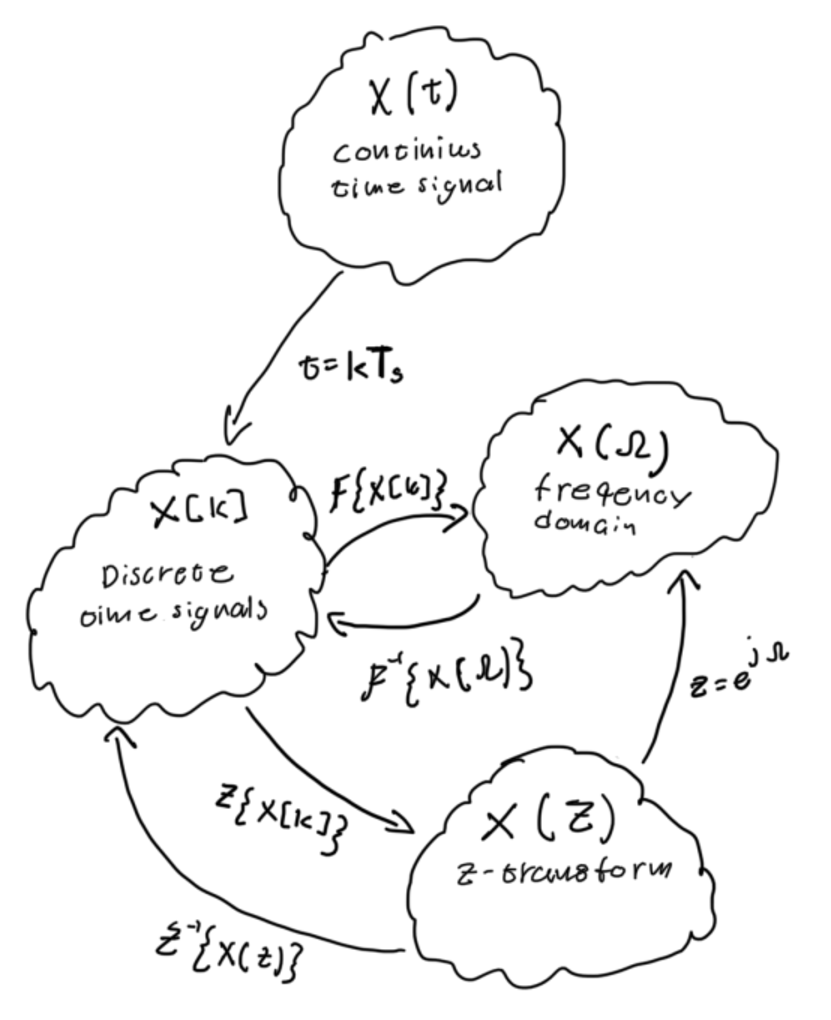
\includegraphics[width=8cm]{image/connection_mind-map.pdf} 
   \caption{Connection mind map.}
   \label{fig:connection_mind-map}
\end{figure}


\begin{exampleblock}{Example: sine in sine out for discrete time signal}
    The sampling time is $T_s = 0.05$ 
    \begin{equation*}
        x(t) = 0.25\cos(2\pi/4 10 t) \Rightarrow x[k] = 0.25\cos(2\pi/4 10 k T_s) = 0.25\cos(\pi/4 k)
    \end{equation*}

    \begin{equation*}
        H(\Omega) = H(z)|_{z=e^{j\Omega}} = \frac{ 1 -0.8e^{-j\Omega} +0.16e^{-2j\Omega} }{ 1 -e^{-j\Omega} +0.5e^{-2j\Omega} } \;\;\; \text{ Where } \Omega_0 = \frac{\pi}{4}
    \end{equation*}

    \begin{align*}
        |H(e^{j\pi/4})| &= 1.7  \\
        \angle H(e^{j\pi/4}) &= 0.14 \;\;\; (7.8^{\circ})
    \end{align*}

    \begin{equation*}
        y[k] = 0.4\cos(\frac{\pi}{4}k + 0.14)
    \end{equation*}
\end{exampleblock}
    

\begin{appendices}
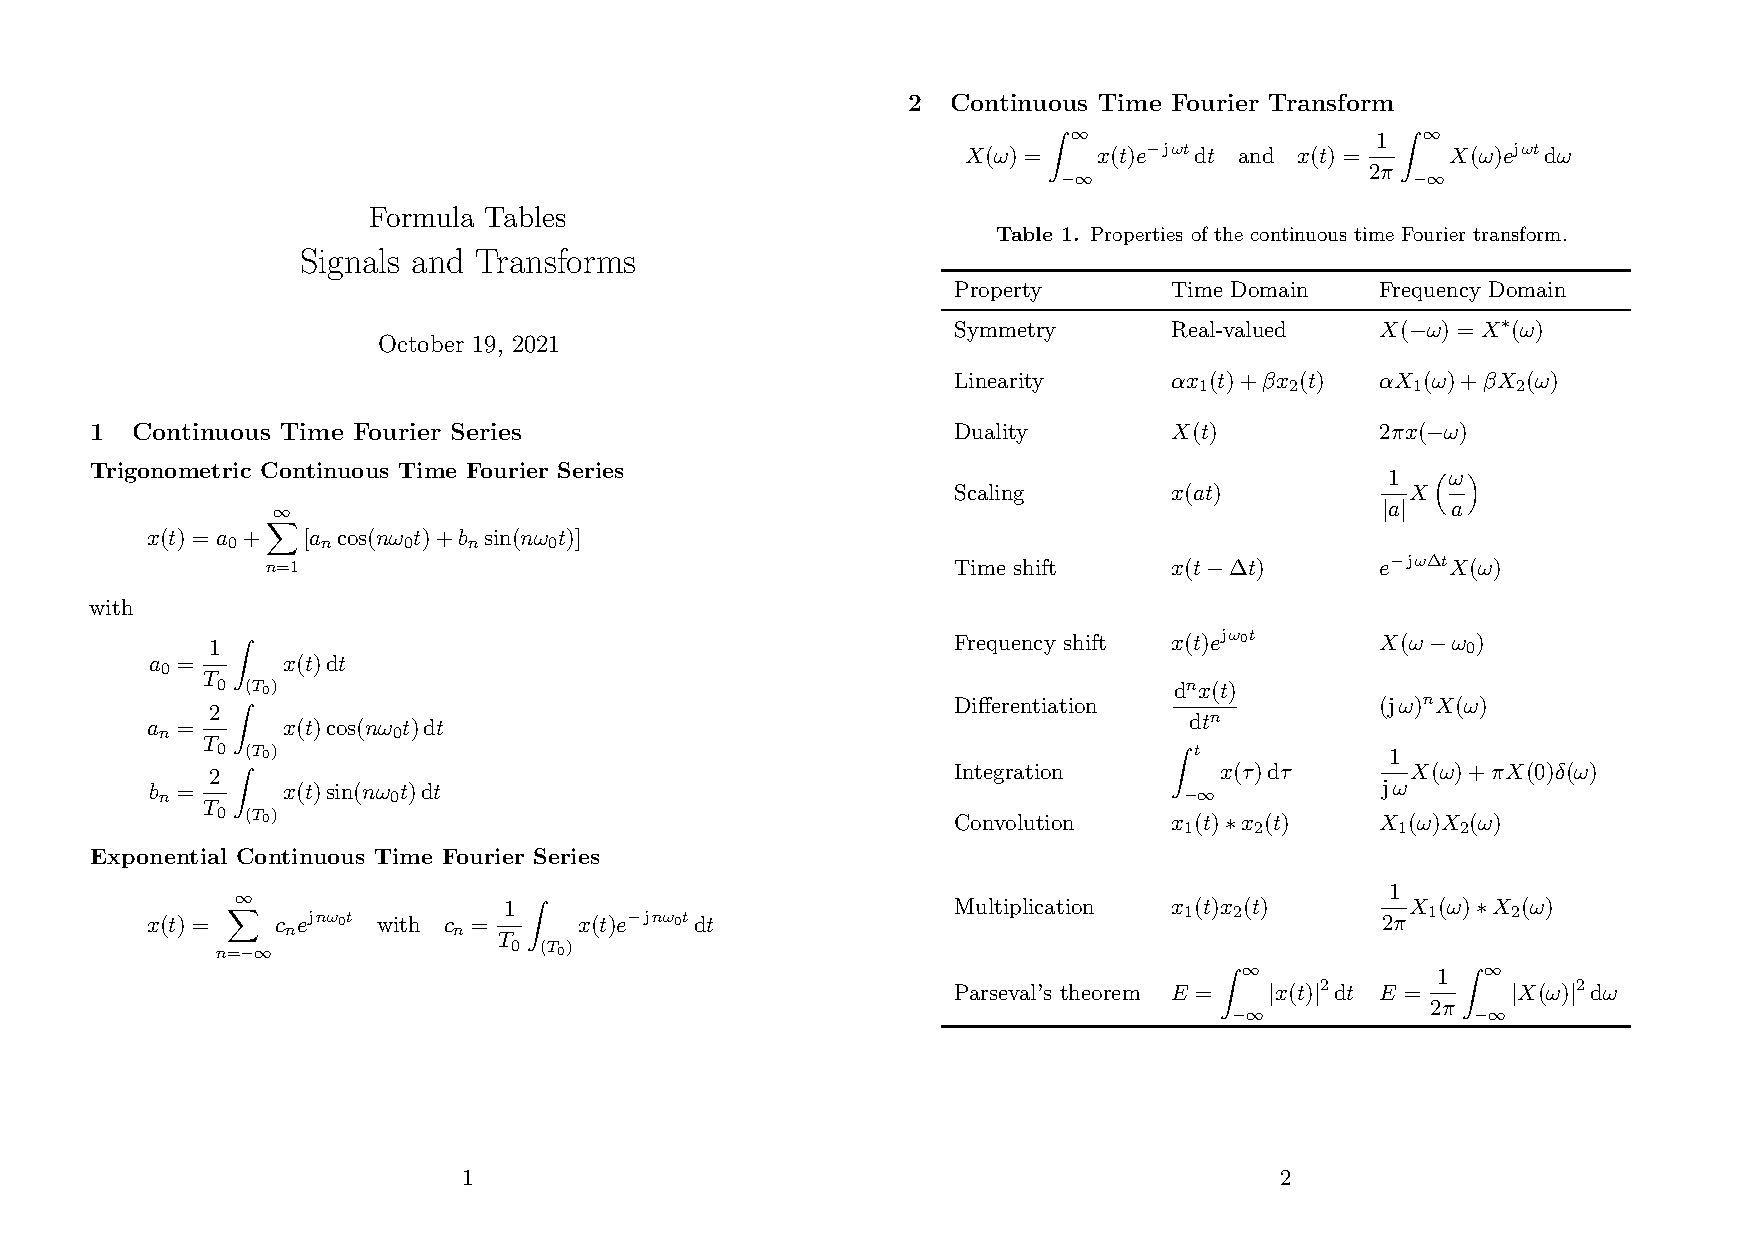
\includepdf[pages=-,pagecommand={},width=\textwidth]{image/transform_tables.pdf}
\begin{figure}[H]
   \centering
   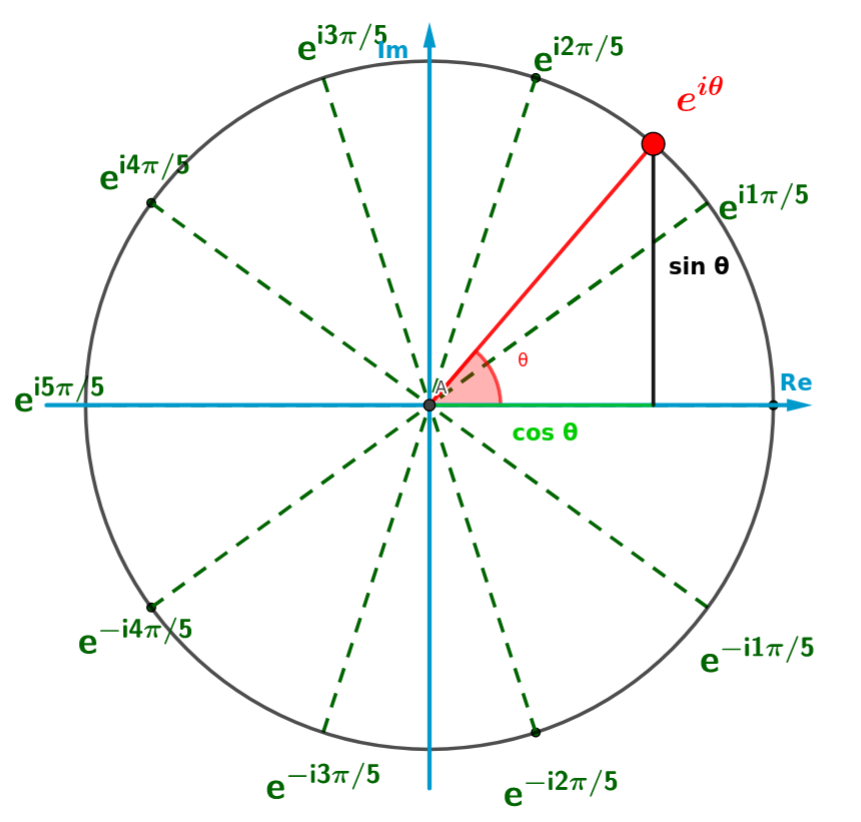
\includegraphics[width=12cm]{image/complex_unit_circle.png} 
   \caption{Complex unit circle. From \cite{st}}
   \label{fig:complex_unit_circle}
\end{figure}
\end{appendices}